%%%%%%%%%%%%%%%%%%%%%%%%%%
\chapter{MATERIALS AND METHODS} \label{chap:3}
%%%%%%%%%%%%%%%%%%%%%%%%%%
\def\etal{{\it et al.}\/}
%%%%%%%%%%%%%%%%%%%%%%%%%%
\section{Introduction}
%%%%%%%%%%%%%%%%%%%%%%%%%%
\begin{sloppypar}
Materials are mainly found in three phases; solids, liquids and gases. Most of the molecular/atomic properties of materials are based on their existing phase. In gaseous phase, the molecules are at long distance and arranged in random manner. Thus the material density and intermolecular interaction is low at the normal temperature and pressure~\citep{Frenkel2002}. The molecules in liquid phase have only short-range arrangement 
and density is larger than that in gaseous phase. The interatomic/molecular interactions in liquids is stronger than to those in gaseous phases, respectively. In solids, the atoms or/and molecules have long-range arrangement with the highest atomic packing. This causes the highest density and the strongest interaction in between the constituent particles. Based on these properties, it is understood that the arrangement of the particles and nature of their interaction differ from one phase to another~\citep{Hansen2006}. Also the properties of interest are size and dimensionality dependent~\citep{Rao2009}. In this context, one can consider the atomistic level of study to understand the microscopic properties of a material where the separate identity of electrons is neglected. For nanostructures, however, diagnosis of electronic properties is essential to understand their basic physics and chemistry. Hence the basic techniques to study their properties differ on the basis of their atomic/molecular arrangement and properties of interest.
\end{sloppypar}

In the present work, we study the structural and transport properties of nitric oxide, alkali-halide ions in water  using empirical potential from molecular dynamics simulation technique at diffrent tempeartures. Then, We discuss the transport and thermodynamic properties of light alkanes (methane, ethane, propane and n-butane) in water. In addition, we perform  the atomistic level of calculations by incorporating empirical force field for the study of free energy of solvation of light alkanes in different liquid media (water, methanol and ethanol). In this chapter, we begin our discussion from the theoretical background and then move into the systems considered for the present work. 

\begin{enumerate}[(a)]
\item Many physically-based numerical simulations model easily observable real world phenomena.
 
\item Molecular Dynamics (MD) simulations model things that are too small for us to observe directly.
\item Modeling the motion of a complex molecular problems and solving the problems by  the 
wave-function and density-functional theory methods of calculations would be accurate. But it would also be very difficult to program and take more computing power than anyone has.  Therefore, we can not use quantum mechanical methods to solve the larger or complex systems. 
\item Instead of using Quantum Mechanics, we can use classical Newtonian mechanics to model our system.
This is a simplification of what is actually going on, and is therefore less accurate. To alleviate this problem, we use numbers derived from quantum mechanical calculations or ab-initio calculations for the constants in our classical equations.
\item  Molecular dynamics (MD) is 
numerical method for studying many-particle systems such as molecules, clusters, and even macroscopic systems such as gases, liquids and solids. It is 
used extensively in materials sciences, chemical physics, and biophysical-chemistry.
\end{enumerate}

A material is made up of a large number of atoms and/or molecules, where an atom (the smallest building block of a material) contains a positively charged nucleus at the center and light electrons in the shells around the nucleus. The number, distribution, and the interactions in between electrons and also with the nucleus in addition to the inter-atomic/molecular bonding determine the electronic properties of a material. The electronic structure of a material consisting of many interacting nuclei and electrons can thus be described by the quantum mechanical treatment of many body Schr\"onger equation \citep{Martin2004}. 

%%%%%%%%%%%%%%%%%%%%%%%%%%
\section{Statistical Mechanics and  Ensembles} 
%%%%%%%%%%%%%%%%%%%%%%%%%%
Statistical Physics is the study of the special laws which govern the behavior and properties of macroscopic systems (that is, systems formed of a very large number of individual particles, such as atoms and molecules). To a substantial limit the general character of these laws does not depend on the mechanics (classical or quantum) which describes the motion of the individual particles in a body, but their confirmation asks a different argument in the two cases. In principle, we can obtain complete information concerning the motion of a mechanical system by constructing and integrating the equations of motion of the system, which are equal in number to its degrees of freedom. On the other hand,  if we consider a system which has a very large number of degrees of freedom, the actual application of the methods of mechanics demands the setting up and solving the same number of differential equations, which in general is not applicable. It should be stressed that it would be completely impossible to substitute in the general solution the initial conditions for the velocities and coordinates of all the particles, even if we could integrate these equations in a general form. That means, we can conclude that as the number of particles increases, the complexity and intricacy of the properties of the mechanical system increases, and  no trace of regularity can be found in the behavior of a macroscopic system. Thus, even though the motion of systems with a very large number of degrees of freedom obeys the same laws of mechanics as that of systems consisting of a small number of particles, the existence of many degrees of freedom results in laws of a different kind. The importance of statistical physics in many other branches of theoretical  physics is due to the fact that in Nature we continually encounter macroscopic bodies whose behavior can not be fully described by the methods of mechanics alone, for the reasons mentioned above, and which obey statistical laws ~\citep{Landau1980}.
\begin{sloppypar}
In Statistical Physics, system under consideration can be studied with few macroscopic properties such as temperature (T), pressure (P) and volume (V). If these three quantities have uniform value we can state that we have one macroscopic realization of a system. On the other hand, this state can be achieved through numerous microscopic realizations of the system. Molecules in a system can have for example same average velocity in many different ways. Gibbs introduced the idea of a statistical ensemble to describe a macroscopic system.\\
 A state of a system under consideration can be specified by the 3N canonical
coordinates $q_1,..., q_{3N}$ and their conjugate momenta $p_1,..., p_{3N}$. The 6N-dimensional space spanned by ${\{q_i, p_i} \}$ is called the $\Gamma$-space, or phase space, of the system. A point in $\Gamma$-space  represents a state of the entire N-particle system, and is referred to as the representative point. Over the time system will pass through multiple points and it will draw a trajectory in phase space. This trajectory is something we could be able to calculate if only we had capabilities to solve $\vec{F} =m\vec{a} $ with adequate initial conditions for all particles under consideration. After long period of time, system will visit every point in phase space although some of the points will be less accessible. To deal with all this we use ensembles. Their description that we like best is maybe the one given by Gibbs who states that ``ensemble is a collection of systems, identical in composition and macroscopic condition but existing in different states''. According to Gibbs, an ensemble is geometrically represented by a distribution of representative points in $\Gamma$-space, usually a continuous distribution, a density function $\rho$(p, q, t). The density function $\rho(p, q, t)$,  is so defined that $\rho(p, q, t)$ $d^{3N}p~d^{3N}q$, is the number of representative points that at time $t$ are contained in the infinitesimal volume element $d^{3N}p~d^{3N}q$ of $\Gamma$-space centered about the point $(p, q)$, with  $(p, q)$ is an abbreviation for ($p_1$,..., $p_{3N}$; $q_1$,..., $q_{3N}$). It is to be emphasized that members of an ensemble are mental copies of a system and do not interact with one another ~\citep{huang2009}.\\ 
Given $\rho (p, q, t)$ at any time $t$, its subsequent values are determined by the dynamics of molecular motion. Let the Hamiltonian of a system in the ensemble be ${H}$($p_1$,..., $p_{3N}$; $q_1$,..., $q_{3N}$. The equations of motion for a system are given
by
\begin{eqnarray}\label{hamiltonian}
\dot{p_i} = -\frac{\partial {H}} {\partial q_i}~~~ (i = 1, 2  ...., 3N)\nonumber\\
\dot{q_i} = \frac{\partial {H}} {\partial q_i}~~~ (i = 1, 2  ...., 3N) 
\end{eqnarray}
Eq. (\ref{hamiltonian}) describes us   how a representative point moves in $\Gamma-space$ as time evolves. When we assume that the Hamiltonian does not depend on any time derivative of $p$ and $q$, the Eq. (\ref{hamiltonian} is invariant under time reversal and uniquely determines the motion of a representative point for all times, when the position of the representative point is given at any time. It follows immediately from these observations that the locus of a representative point is either a simple
closed curve or a curve that never intersects itself. Furthermore, the loci of two distinct representative points never intersect ~\citep{huang2009}.\\
The aim of statistical mechanics is to derive all the equilibrium properties of
a macroscopic molecular system from the laws of molecular dynamics. Thus it
aims to derive not only the general laws of thermodynamics but also the specific
thermodynamic functions of a given system. Classical statistical mechanics is founded on the following postulate.
\begin{enumerate}
\item \textbf{Postulate of Equal a Priori Probability} ~~~~~  When a macroscopic system is in
thermodynamic equilibrium,  its state is  equally likely to be any state satisfying the macroscopic conditions of the system.
\item \textbf{Ergodicity } ~~~~~~ The ensemble average  of a measurable property of the system, such as energy or momentum, say $f(p,q)$ in thermodynamic system of interest is equal to the time average  of $f(p,q)$ taken over a long time interval.
\end{enumerate}
The ensemble average of $f(p, q)$ is defined by
\begin{equation}
\left\langle f \right\rangle_{ensemble} = \frac{\int d^{3N}p~ d^{3N}q~ f(p, q)~ \rho (p,q)} {\int d^{3N}p~ d^{3N}q~ \rho (p,q)}
\end{equation}
The time average of  $f(p, q)$ is defined by 
\begin{equation}
\left\langle f \right\rangle_{time} = \lim_{t\to\infty} \frac{1}{t} \int_{0}^{t} f(p, q) ~ dt
\end{equation}
In MD simulations, solving the physical problems on a computer, for large number of particles, the experimentally observable macroscopic property $f_{obs}$ can be written as \citep{huang2009, Allen1989}
\begin{equation}
 f _{obs} = \left\langle f \right\rangle_{ensemble} = \left\langle f \right\rangle_{time}
\end{equation}
\end{sloppypar}
Time average and ensemble average are usually taken as the same thing but that  doesn't need to always be true. If a system has this property it's said to be ergodic, and equivalence of time and ensemble averages itself is called ergodicity. Ensemble is then assembly of all possible micro-states that can be achieved by a system under imposed macroscopic conditions. Ensembles can be divided according to macroscopic quantities that hold constant value. Some of the common  types of ensembles are:

\begin{itemize}
\item Microcanonical ensemble (N, V, E)
\item Canonical ensemble (N, V, T)
\item Grand canonical ensemble ($\mu$, V, T)
\item  Isothermal-isobasic - ensemble (N, P, T)
\item Isoenthalpic-isobaric -  ensemble (N, P, H)
\end{itemize}

\begin{figure}[h!]
\centering
\includegraphics[width=15.5cm,height=5.5cm]{Chapter3/Statistical_Ensembles.png}
\caption {Visual representation of different statistical ensembles. (https://en.wikipedia.org/wiki/Statistical Ensemble (mathematical physics), dated: May 5, 2018).}  
\end{figure}
%%%%%%%%%%%%%%%%%%%%%%%%%%
\subsection{Microcanonical Ensemble} 
%%%%%%%%%%%%%%%%%%%%%%%%%%
This ensemble represents all states that have fixed total energy, number of particles and volume. That means in this ensemble the macrostate of a system is defined by the number of molecules $N$, the volume $V$ and the energy $E$. However, from a practical point of view, an absolutely isolated system is too much of an idealization and its energy cannot be defined sharply.  Therefore, in the microcanonical ensemble every system has $N$ molecules, a volume $V$, and an energy between $E$ and $E + \Delta$, $\Delta \ll  E $. Now, the microcanonical ensemble is a collection of systems for which the density function $\rho $  is given by \citep{huang2009, pathria1996}:
\begin{eqnarray}
\rho (p,q)= \begin{dcases}
    Const. & \text{if }  E \leq H(p,q)\leq  E+ \Delta \\
    0,              & \text{otherwise}
\end{dcases} 
\end{eqnarray}
The fundamental quantity that furnishes the connection between the microcanonical ensemble and thermodynamics is the entropy. It is the main task of this section to define the entropy and to show that it possesses all the properties attributed to it in thermodynamics.\\
Let $\Gamma(E) $  and  $\Sigma (E)$  denote the volume in $\Gamma $ space occupied by the microcanonical ensemble and  the volume in $\Gamma $ space enclosed by the energy surface of energy $E$ respectively: 
\begin{align}
\Gamma(E) &= \int_{E \leq H(p, q)\leq  E+ \Delta} d^{3N}p~ d^{3N}q  \\
\Sigma (E) & = \int_{ H(p, q)\leq  E } d^{3N}p~ d^{3N}q 
\end{align} and then 
\begin{equation}
\Gamma(E) = \Sigma (E + \Delta ) - \Sigma (E) 
\end{equation}
If $\Delta $ is so chosen that $\Delta \ll E $, then
\begin{equation}
\Gamma(E) = \omega (E) ~ \Delta
\end{equation}
where $\omega(E)$ is called the density of states of the system at the energy $E$ and is
defined by 
\begin{equation}
\omega(E)= \frac{\partial \Sigma (E)}{\partial E}
\end{equation}
 The entropy is defined by the following relations which are equivalent to each other 
 \begin{align}
 S &= k_B~log~\Gamma(E) \nonumber \\
 S &= k_B~log~\omega(E) \\
 S &= k_B~log~\Sigma(E) \nonumber
 \end{align}
 where, $k_B$ is is a universal constant,  Boltzmann's constant. \\
 Other thermodynamic quantities, absolute temperature (T),  pressure (P), internal energy (U), Helmholtz free energy (A), Gibbs free energy (G), heat capacity at constant volume ($C_V$), can be obtained from entropy with use of Maxwell thermodynamical  relations \citep{huang2009}: 
 \begin{align}
  U (S, V)& = E (S, V) \nonumber \\
    T & = \left(  \frac{ \partial U} {\partial S }\right)_V  \nonumber \\
   P  &  = - \left(  \frac{ \partial U} {\partial V }\right)_S  \\
    A & = U - T~S \nonumber \\
     G & = A + P~ V = U + P~V - T~ S \nonumber\\
     C_V & = \left(  \frac{ \partial U} {\partial T }\right)_V  \nonumber
 \end{align}
%%%%%%%%%%%%%%%%%%%%%%%%%%
\subsection{Canonical Ensemble} 
%%%%%%%%%%%%%%%%%%%%%%%%%%
Canonical ensemble represents a system that has constant number of particles, size and temperature. It is an ensemble in which  the macrostate of a system is defined by the number of molecules $N$, the volume $V$ and the temperature energy $T$. A canonical  ensemble is appropriate for the description of a system not in isolation, but in thermal equilibrium with a larger system.  The  canonical ensemble describes those systems which are not isolated but are in thermal contact with the heat reservoir under consideration together with a heat reservoir forms a closed system and then the system of interest is treated as a subsystem of the closed system. For the canonical ensemble,  the density function $\rho $  is given by \citep{huang2009}: 
\begin{equation}
\rho (p, q) = e^{-\beta H(p,~ q)} 
\end{equation} 
where $\beta = 1/k_B~T$ and $H(p, q)$ is the Hamiltonian of the system. The volume in $\Gamma$ space occupied by the canonical ensemble is called the canonical partition function $Q_N(V, T)$:
\begin{equation}
Q_N(V, T) = \frac {1}{N! h^{3N}}\int d^{3N}p~ d^{3N}q ~ e^{-\beta H(p,~ q)}  
\end{equation} 
Connection with thermodynamics for this system is Helmholtz free energy $A (V, T)$, which is obtained from the formula: 
\begin{align}
Q_N(V,~T) & = e^{-\beta~A(V,~T)}\nonumber\\
or, ~~ A(V,~T) &= k_B~T~log~Q_N(V,~T)
\end{align}
All other thermodynamic functions may be found from $A(V, T)$ by the Maxwell relations in thermodynamics:
\begin{align}
   S & = -\left(  \frac{ \partial A} {\partial T }\right)_V  \nonumber \\
   P  &  = - \left(  \frac{ \partial A} {\partial V }\right)_T \nonumber \\
   G & = A + P~ V \\
   U &= \left\langle  H \right\rangle  = - \frac{\partial} {\partial \beta } log Q_N(V,~T) = A + T~S \nonumber \\
   \mu & = \left(  \frac{ \partial A} {\partial N }\right)_V \nonumber
 \end{align}
%%%%%%%%%%%%%%%%%%%%%%%%%%
\subsection{Isothermal-Isobaric  Ensemble} 
%%%%%%%%%%%%%%%%%%%%%%%%%%
This ensemble depicts systems with constant pressure, temperature and number of particles. It is an ensemble in which  the macrostate of a system is defined by the number of molecules $N$, the pressure $P$ and the temperature energy $T$. It is of great importance since these conditions are valid for a large number of systems and it is widely used. We can picture it as a small system inside a big reservoir that keeps its pressure and temperature constant. Constant pressure means that the volume of a system is changing through time. For the isothermal-isobaric ensemble, the density function $\rho $ is given by \citep{Allen1989}: 
\begin{equation}
\rho (p, q) = e^{-\beta(H + P~V)} 
\end{equation} 
where $\beta = 1/k_B~T$ and $H(p, q)$ is the Hamiltonian of the system. The isobaric-isothermal   partition function $Q_{NPT}$:
\begin{equation}
Q_{NPT} = \frac {1}{N! h^{3N}} \int d^{3N}p~ d^{3N}q ~dV ~ e^{-\beta(H + P~V)}  
\end{equation} 
Connection with thermodynamics for this system is Gibbs free energy $G$, which is obtained from the formula: 
\begin{align}
G & = - k_B~T~log~Q_{NPT} = A + P~V
\end{align}
%%%%%%%%%%%%%%%%%%%%%%%%%%
\section{Structural, Transport and Thermodynamic Properties}
%%%%%%%%%%%%%%%%%%%%%%%%%%

A system is not in equilibrium when the distribution function is different from the Maxwell-Boltzmann distribution. The most common case of a nonequilibrium situation is that in which the temperature, density, and average velocity are not constant throughout the system. To approach equilibrium, these nonuniformities have to be resolved through the transport of energy, mass, and momentum
from one part of the system to another. In MD simulations, we wish to measure interesting properties of many-body systems that can be compared with real experiments. Those properties   include structural, transport, and  thermodynamic properties. The structural properties of the fluid mixture is analyzed by using radial distribution function (RDF). The transport properties includes the physical properties such as  diffusion coefficients, shear viscosity, thermal conductivity, mobility, friction coefficients. The thermodynamic properties of the system under consideration includes the thermodynamical physical quantities such as Temperature $T$, the pressure $P$, the specific heat capacity $C_V$, Gibbs free energy $G$, Helmholtz free energy $A$. The thermodynamic properties also includes free energy of solvation, chemical potential $\mu$ ~\citep{huang2009, Frenkel2002}. In the following section, we  discuss the radial distribution function (RDF), phenomenon of diffusion and diffusion coefficients, free energy of solvation and method of calculations.
\end{sloppypar} 
%%%%%%%%%%%%%%%%%%%%%%%%%%
\subsection{Radial Distribution Function (RDF)}
%%%%%%%%%%%%%%%%%%%%%%%%%%
\begin{sloppypar}
The relative arrangements of atoms and molecules in fluid and solid phases are most often accurately described in terms of the principles of classical statistical mechanics. There are, of course, electrons surrounding the nuclei in these systems, and the behavior of electrons is surely quantum mechanical in nature. Yet after averaging over these quantal fluctuations, the remaining problem is to sample the statistical configurations of the nuclei in the effective interactions induced by the electrons we have already integrated out~ \citep{chandler1987}.\\
Molecular structure refers to the patterns and correlations that molecules display in
their placement in space. Molecules are in constant motion, rotating and moving about in erratic ways, so the notion of structure has meaning only in average sense. There
are many ways to quantify this average structure, one of them is estimation  of radial distribution function. The structure of a simple fluid is characterized by a set of distribution functions for the atomic positions, the simplest of which is the pair distribution function $g(\mathbf{r})$. This function gives the probability of finding a pair of atoms at distance $r$ apart, relative to the probability expected from a completely random distribution at the same density. The pair distribution function $g(\mathbf{r})$ is most simply thought of as the  number of atoms at distance r from a given atom compared with the number at the same distance in an ideal gas at the same density. For an isotropic system, the pair distribution function is a function of only the separation of atoms $r = \lvert\mathbf{r}\rvert $, and is completely defined by the radial distribution function (RDF), denoted by $g(\mathbf{r})$ ~ \citep{Allen1989}. The radial distribution function describes how, on average, the atoms in a system are radially packed around each other.\\
For a system of fluid of  $N$ particles, volume $V$ and temperature $T$, with density of fluid $\rho = N/V$, the definition of the radial distribution function, g(r),
infers that $\rho g(r)~d\mathbf{r}$ is the probability of observing  a second molecule in d$\mathbf{r}$  given that there is a molecule at the origin of $\mathbf{r}$. This probability is not normalized to unity, but we have 
\begin{equation}\label{rdf}
\int_0^\infty \rho g(r)~4\pi r^2~dr = N-1 \approx N
\end{equation}
The Eq. (\ref{rdf}) shows that $\rho g(r)~4\pi r^2~dr $   is the number of
molecule between $r$ and $r + dr$ about a central molecule. When the bulk density $\rho$ is multiplied by the factor $g(r)$, we obtain the  local density $\rho(r) = \rho g(r)$. Since molecules become effectively hard  as $r \longrightarrow 0$, $g \longrightarrow 0$ as $r \longrightarrow 0$. Also, since the influence of molecule at the origin diminishes as r becomes very large, $g \longrightarrow 1$, as $r \longrightarrow \infty$ ~\citep{mcquarrie2000}.
\begin{figure}[h!]
\centering
\includegraphics[width=15 cm,height=11 cm]{Chapter3/coordination.png}
\caption {Simple liquid structure~\citep{chandler1987}.} 
\label{coordinationfig} 
\end{figure}
\begin{figure}[h!]
\centering
\includegraphics[width=14 cm,height=11 cm]{Chapter3/rdf.png}
\caption {The radial distribution function for a simple fluid~\citep{chandler1987}.} 
\label{rdffig} 
\end{figure}
 A schematic view of the liquid structure (drawn in two dimensions for artistic convenience) is shown in Fig. (\ref{coordinationfig}), which shows the most probable location of first and second coordination shell with respect to a fixed molecule. In the figure, $\sigma$ is the van der Waals diameter (which is roughly equal to  the distance of closest approach between two atoms during a physical  encounter), the cross-hatched atom is the reference atom which is at the origin. The atoms are drawn close  together because of typical liquid densities, and  Since the fluid is  dense, there is a strong likelihood that a first neighbor shell will be  found around $r = \sigma$. The nearest neighbors, which comprise the \textit{first  coordination shell}, tend to exclude the next nearest neighbors from
 an intermediate region around $r = 1.5 \sigma$ and  $g(r)$ will be less than 
 unity in that region, and it will peak above the uncorrelated result 
 near $r = 2\sigma$. The RDF of a liquid and gas phase of argon is shown in Fig. (\ref{rdffig}). For, the  liquid, the second peak corresponds to the most probable
 location for the next nearest neighbors and these neighbors comprise  the \textit{second coordination shell}. This layering manifests the granularity  (non-continuum nature) of the liquid. It shows up in an oscillatory  form for g(r), which persists until r is larger than the range of  correlations (typically a few molecular diameters in a dense liquid). 
 In the dilute gas phase, the range of correlations is just the range of
 the intermolecular pair potential and there is no layering.   Notice both in the  Fig. (\ref{coordinationfig}) of the liquid  and the Fig. (\ref{rdffig}) of g(r)  that there is a finite density of particles even in ''unlikely'' regions  like $r = 1.5 \sigma $. This is one of the features that distinguishes a liquid from a crystalline solid. Without it, the possibility of diffusion would  be drastically reduced. In crystalline solids, RDF shows sharp peaks and troughs up to infinity where the separations and heights are  the characteristics of the lattice structure. In liquids however, RDF oscillates up to  certain orders and then attains constant value as unity~\citep{chandler1987, mcquarrie2000}\\
 The radial distribution function or pair distribution function $g_{AB}(r)$ between particles of type $A$ and $B$ is defined in the following way~\citep{Gromacs-manual}: 
 \begin{equation}
 g_{AB}(r) = \frac{\langle \rho_B (r) \rangle}{\langle \rho_B \rangle_{local}} = \frac{1}{\langle \rho_B \rangle_{local}} \frac{1}{N_A}  \sum_{i\in A}^{N_A} \sum_{j\in B}^{N_B} \frac{\delta(r_{ij}-r)}{4\pi r^2}
  \end{equation}
  where $\langle \rho_B (r) \rangle$ is the particle density of type $B$ at a distance $r$ around particles $A$ and  $\langle \rho_B \rangle_{local}$ is the particle density of type $B$ averaged over all the spheres around particles  $ A$.
  \end{sloppypar} 
  The radial distribution function turns out to be of central importance in the theory of liquids for two reasons. First, all the thermodynamic functions can be written in terms of $g(r)$ if we assume the total potential energy of the N-body system is pairwise additive: 
  \begin{equation}
 U_N(r_1, r_2, ..., r_N) = \sum_{i<j} u(r_{ij})
 \end{equation}
 In addition, the radial distribution function can be determined by diffraction studies on liquids. In a solid the molecules are arranged regular repeating order and this leads to a sharp X-ray diffraction pattern from which the order of molecules in solid can be obtained. The X-ray diffraction pattern of liquid is more diffuse but can be used to determine the local short-range order in a fluid as depicted in Fig. (\ref{rdffig}). The peaks in the curve represent the smeared-out shells of first nearest neighbors, second nearest neighbors, etc., which in a sense are remnants of ordering found in the solid ~\citep{chandler1987, mcquarrie2000}. 
 
  %%%%%%%%%%%%%%%%%%%%%%%%%%
  \subsection{Diffusion and Diffusion Coefficient}
  %%%%%%%%%%%%%%%%%%%%%%%%%%
   There are  different transport phenomenon whereby mass, energy, or momentum are transported from one region of a material to  another under the influence of composition, temperature, or velocity gradient.
 Diffusion refers to the the movement of matter within a single phase from a region of high concentration to a region of low concentration in the absence of mixing. In diffusion, there
 is a net transfer of diffusing particles from the region of higher concentration to the
 region of lower concentration as a result of random molecular motions. This definition of diffusion is fundamental throughout science, from gas exchange in the lungs to the spread of carbon dioxide in the atmosphere to the movement of water from one side of a cell's plasma membrane to the other. However, the concept of diffusion is rarely as simple as molecules moving from one place to another. Temperature, the size of the molecules involved, the distance molecules need to travel, the barriers they may encounter along the way, and other factors all influence the rate at which diffusion takes place ~\citep{cussler2009}. 
  \begin{figure}[h!]
  \centering
  \includegraphics[width=14cm,height=6cm]{Chapter3/diffusion.jpg}
  \caption {Cartoon of diffusion of a purple dye in water.  (https://www.visionlearning.com/en/library/Chemistry/1
  /Diffusion-I/216, dated: May 14, 2018)}
  \label{diffusion} 
  \end{figure}
    A simple illustration of this process can be seen using a glass of water and food coloring. When a drop of food coloring enters the water, the food coloring molecules are highly concentrated at the location where the dye molecules meet the water molecules, giving the water in that area a very dark color (Figure \ref{diffusion}). The bottom of the glass initially has few or no food coloring molecules and so remains clear. As the food coloring molecules begin to interact with the water molecules, molecular collisions cause them to move randomly around the glass. As collisions continue, the molecules spread out, or diffuse, over space. Eventually, the molecules spread throughout the entire glass, becoming evenly distributed and filling the space. At this point, the molecules have reached a state of equilibrium in which no net diffusion is taking place and the concentration gradient no longer exists. In this state, the molecules are still moving haphazardly and colliding with each other; we just can't see that motion because the water and color molecules are evenly dispersed throughout the space. Once equilibrium has been reached, the probability that a molecule will move from the top to the bottom is equal to the probability a molecule will move from the bottom to the top.
    \end{sloppypar}
    \subsubsection{Self Diffusion}
        The diffusion in a homogeneous system with no chemical concentration gradient is known as self diffusion. The corresponding diffusion coefficient is called the self-diffusion coefficient. For an instance, the water molecules even in pure water are in continuous random motion; their migration through the liquid is a perfect example of self-diffusion. It is a simple form of diffusion where the diffusing species are identical to one another in every aspect ~\citep{mehrer2009, heitjans2006}.\\
        \noindent There are two common ways to obtain a self-diffusion coefficient. The
        first is from the positions of all the molecules present in the system and the second
        is from velocity of each molecule in the system. The mathematical expression to
        calculate self-diffusion coefficient from molecular positions is famously known as
        Einstein relation. The diffusion coefficient calculated using velocities information is known as Green-Kubo formalism, and was first established by Green and Kubo. The Einstein's relation and the Green-Kubo formalism should give identical results. The methods using Einstein relation and  Green-Kubo formalism  are, respectively, called as mean square displacement (MSD) and velocity autocorrelation function (VACF) methods.  In Einstein MSD method, self diffusion coefficient is obtained from the evaluation of  mean-square displacement of particles obtained using simulated trajectories of the particles. In the VACF method, the self diffusion coefficient is obtained by integrating the velocity auto-correlation function~\citep{Allen1989, Frenkel2002}.     
    \subsubsection{Binary or Mutual Diffusion}
    In a system containing two different species, binary or mutual diffusion takes place
    due their mass movement in the system and the corresponding diffusion coefficient is
    called binary or mutual diffusion coefficient. The self-diffusion coefficients of these
    two species are related to the mutual diffusion coefficient of their binary mixture by
    the Darken's phenomenological relation~\citep{darken1948}:
    \begin{equation}
    \label{darken}
    D_{12} = N_{2}~D_{1} + N_{1}~D_{2}
    \end{equation}
       where, D$_{12}$ is the binary diffusion coefficient, D$_{1}$ and D$_{2}$ are the self-diffusion coefficients of species $1$ and $2$, respectively and   N$_{1}$  and N$_{2}$  are the corresponding mole fractions.
    \subsubsection{Mathematical Treatment of Diffusion: Ficks Law and Einstein's Relation}
   The microscopic theories of transfer processes are based on the phenomenological approach in which the basic transfer relations are postulated from experience without reference to the details of mechanism of transfer. By definition, a transfer process  consists of net flow of a property under the influence of driving force. The rate of transfer is the flux and the intensity of driving force is the  gradient (concentration, velocity, pressure, temperature, or potential). The 
   transfer process (or flux) takes place in the direction of decreasing of the driving force that is gradient~\citep{bird2002}. The flux and the gradient are related by a phenomenological relation of the form:
   \begin{equation}
   \mathrm{Flux} = -\mathrm{coefficient} \times \mathrm{gradient}
   \end{equation}
   where, the coefficient characterizes the resistance to the transfer or flow.\\
    The macroscopic law that describes the diffusion is known as  Fick's first law which states that the flux  $\mathbf{J}$ of the diffusing species is proportional to the negative gradient in the concentration of the species \citep{Frenkel2002}: 
    \begin{equation}
    \label{fickslaw}
    \mathbf{J} = -D\nabla C(\mathbf{r},t)
    \end{equation}      	  						     	 	          
    where  $D$, the constant of proportionality, is referred to the \textit{diffusion coefficient} or the \emph{diffusivity}, and has dimensions $(length)^ 2 (time)^{-1}$. The concentration gradient vector $\nabla C(\textbf{r},t)$ points in that direction for which the concentration field undergoes the most rapid increase. The negative sign in Eq.(\ref{fickslaw}) indicates that the particle flux is directed opposite in direction to the concentration gradient vector. It is to be noted  that Eq.(\ref{fickslaw}) is valid only for an isotropic medium. The flux $\textbf{J}$ is normal to the equi-concontration surface, inforced by the assumption of isotropic symmetry in the medium~\citep{crank1979}. Diffusion of a labeled species among otherwise identical solvent molecules is called \textit{self-diffusion.} The Fick’s first law for the flux of diffusing particles in one direction (x-direction) is illustrated in figure \ref{diffusion_ficks}.
     \begin{figure}[h!]
      \centering
      \includegraphics[width=14cm,height=6cm]{Chapter3/ficks.png}
      \caption {Illustration of Fick’s law in one dimension ~ \citep{mehrer2007} } 
      \label{diffusion_ficks} 
      \end{figure}
       In order to know about concentration gradient $\nabla C(\textbf{r},t)$ and hence the diffusion current $\textbf{J}$, we have to compute concentration profile $C(\textbf{r}, t)$ of a diffusing species.  There are several ways to find concentration profile and one of them starts with assumption that at the begining $(t=0)$, all of the diffusing species was concentrated at the origin of our coordinate frame. To compute the time evolution of the concentration profile, we must combine Fick's law with continuity equation of the diffusing species~\citep{mehrer2007}:  
    \begin{equation}
    \label{EoC}
    \frac{\partial C(\mathbf{r},t)}{\partial t} +   \nabla . \mathbf{J} = 0
    \end{equation}
    Exploiting (\ref{fickslaw}) in (\ref{EoC}), we end up with 
    \begin{equation}
    \label{pde}
    \frac{\partial C(\textbf{r},t)}{\partial t} -  D \nabla^2C(\textbf{r},t) = 0
    \end{equation}
    
    Mathematically, $C(\textbf{r},0) = \delta(\textbf{r})$, where $\delta(\textbf{r})$ is Dirac-Delta function.\\
        \noindent Imposing conservation of particle number
    Equation (\ref{pde}) is a partial differential equation, second order in position co-ordinate and first order in time co-ordinate. This equation is linear if $D$ does not depend on concentration (for an instance, diffusion in ideal solid solutions), and it is non-linear if diffusivity depends upon concentration (for an instance, when diffusion due to chemical concentration gradient). Equation (\ref{pde}) is called Fick's second law or diffusion equation.\\
    \noindent Using assumption $C(\textbf{r},0) = \delta(\textbf{r})$, equation (\ref{pde}) yields
    \begin{equation}
    \label{concentration}
    C(\textbf{r},~t) = \frac{1}{(4\pi D t)^{\frac{d}{2}}}~ \exp\left( -\frac{r^2}{4Dt}\right)
    \end{equation}
    where d represents the dimension of the system. For three dimensional system, $d=3$. This is the well-known fundamental solution to the diffusion equation. This equation shows that the diffusing material, which is initially located at the origin, will spread out as a function of time.
    \begin{figure}[h!]
    \centering
    \includegraphics[width=14.4cm,height=6.5cm]{Chapter3/concentrationprofile.png}
    \caption{Concentration profile as a function of time for a diffusing substance which is initially located at the origin~ \citep{mcquarrie2000} }
    \label{fig:concprofile}
    \end{figure}
    
    \noindent Figure \ref{fig:concprofile} depicts the concentration profile of diffusing substance in one dimension (d=1) at different times. As D is constant, plot at different values of Dt represents concentration at different time. It is lucidly seen from figure that as the time passes by the substance distributes more and more homogenously through entire space which once was abudent at origin of co-ordinate axis.\\
    $C(\textbf{r},t)$ satisfies the normalization
    \begin{equation}
    \label{normalization}
    \int drC(\textbf{r},t) = 1
    \end{equation}
    The mean squared displacement (MSD) or the second order moment is defined using concentration profile in following way
    \begin{equation}
    \label{SOM}
    \textless r^2(t) \textgreater = \int drC(\textbf{r},t)r^2
    \end{equation}
    
     To calculate the time evolution of MSD we multiply equation (\ref{concentration}) by $r^2$ and integrae over all space. This yields Then integrating by parts using vector identities and Gauss divergence theorem, we get
    \begin{equation}
    \frac{\partial}{\partial t}\langle r^2(t) \rangle = 6D\int dr C(\textbf{r},t)
    \end{equation}
    As C(\textbf{r},t) is normalized, we end up with
    \begin{equation}
    \label{Einstein}
    D = \frac{1}{6t} \frac{\partial}{\partial t} \langle r^2(t) \rangle
    \end{equation} 
    
    \noindent This is the famous Einstein relation which relates the diffusion coefficient, a macroscopic transport property of the system, with the mean-squared displacement (MSD), a microscopic quantity of the diffusing particles of the system \cite{crank}. As expressed in equation (\ref{Einstein}), the instantaneous diffusion coefficient is given by the slope of a curve of MSD of the diffusive particles versus time. For an MSD that behaves as a straight line after a prolonged period of time, equation (\ref{Einstein}) reduces to
    \begin{equation}
    D = \lim_{t \to \infty} \frac{1}{6} \langle r^2(t) \rangle
    \end{equation}
    \noindent This is the coefficient of self diffusion.
 \subsubsection{Mathematical Interpretation: Fick's Law and Einstein's Relation}
 
 \noindent Let us consider the flux of diffusing particles in one dimension(x-direction) illustrated in Fig.2.1. The particles can be atoms, molecules, or ions. Fick's First law for an isotropic medium can be written as \cite{mehrer},
 \begin{equation}
 \mathbf{J_x} = -D\frac{\partial C(x,t)}{\partial x}
 \label{eqdiff}
 \end{equation}
 
 \noindent Here $J_x$ is the flux of particles(diffusion flux) and C is their number density(concentration). The negative sign in equation (\ref{eqdiff}) indicates opposite directions of diffusion flux and concentration gradient. Diffusion is a process which leads to an equalization of concentation. The factor of proportionality, D, is denoted as the \emph{diffusion coefficient } or as the \emph{diffusivity} 
 of the species considered. Fick's first law is easily generalized to three dimensions using a vector notation \cite{mehrer}: 
              \begin{equation}\label{1}
              \mathbf{J}=-D\nabla{C(r,t)}
              \end{equation}
      
 \noindent The vector of the diffusion flux \textbf{J} is directed opposite in direction to the concentration gradient vector $\nabla{C}$. The Nabla symbol, $\nabla$, is used to express the vector operation on the right-hand side of the equation (\ref{eqdiff}). The nabla operator  acts on the scalar concentration field C(x,y,z,t) and produces the concentration gradient field $\nabla{C}$. The concentration gradient vector always points in that direction for which the concentration  field undergoes the most rapid increase, and it's magnitude equals the maximum rate of concentration at the point. For an isotopic medium the diffusion flux is antiparallel to the concentration gradient.\\
 
 \noindent The diffusion flux is expressed in number if particles (or moles) trasversing a unit area per unit time and the concentration in number of particles per unit volume. Thus the diffusivity \textbf{D} has the dimension of \emph{length$^2$ per unit time } and bears the units [cm$^2$s$^{-1}$] or [m$^2$s$^{-1}$] \cite{mehrer}.\\
 
  For a diffusing species which obeys a conservation law an equation of continuity can be formulated.
 
 \begin{equation}\label{2}
 \frac{\partial C(r,t)}{\partial t} + \nabla . \mathbf{J}(r,t) = 0 
 \end{equation}
 
 \noindent The equation (\ref{2}) is the \emph{continuity equation}. Fick's first law (\ref{1}) and the equation of continuity (\ref{2}) can be combined to give an equation which is called \emph{Fick's second law} or sometimes also the \emph{diffusion equation} \cite{leach}. Combining equation (\ref{1}) and (\ref{2}) we get, 
 
 \begin{equation}\label{3}
 \frac{\partial C(r,t)}{\partial t} = \nabla .(D \nabla C)
 \end{equation}
 \noindent From a mathematical view point Fick's second law is a second-order partial differential equation. To determine the diffusion coefficient of the substance it is necessary to determine the concentration profile of the diffusing substance. One of the several ways to determine the concentration profile is under the assumption that at time t=0, the substance was concentrated at the origin of our coordinate frame, i.e. C(r, 0) = $\delta(r)$.
 
 \noindent From equation (\ref{3}) we get
 
 \begin{equation}\label{4}
 \frac{\partial C(r,t)}{\partial t} -D \nabla^{2} C(r,t) = 0
 \end{equation}
 
 \noindent Equation (\ref{4}) can be solved using the boundary condition
 \begin{equation}
 C(r,0) = \delta(r)
 \end{equation}
 where $\delta(r)$ is the Dirac delta function. This will yield,
 
 \begin{equation}
 C(r,t) =\frac{1}{(4 \pi D t)^{\frac{d}{2}}} \exp{\left(\frac{-r^2}{4 D t}\right)}
 \end{equation}
 
 \noindent where d is the dimensionality of the system. For a three-dimensional system as in our case, it carries a value of $3$.
 
 \noindent To determine the diffusion coefficient the time dependence of second moment of C(r,t) is needed, which is defined as
 
 \begin{equation}\label{7}
 \left\langle r^2(t)\right\rangle \equiv \int d \textbf{r} \; C(r,t)\;r^2 
 \end{equation}
 \noindent where C(r,t) satisfies the normalization condition
  \begin{equation}\label{8}
  \int d\mathbf{r}\;C(r,t) =1
  \end{equation}
 
 \noindent The second moment is also defined as mean-squared displacement (MSD) of the diffusing particles. The time evolution of $\left\langle r^2(t) \right\rangle$ can be obtained by multiplying equation (\ref{3}) by $r^2$ and integrating over all space, which yields
 \begin{equation}
 \int d\textbf{r}\;r^2\;\frac{\partial C(r,t)}{\partial t} = \int d\textbf{r}\; r^2\;D \nabla .(\nabla C(r,t))
 \end{equation}
 \noindent Changing the order of derivative and integration, we get
 \begin{equation}\label{10}
 \frac{\partial}{\partial t}\;\int d\textbf{r}\;r^2\; C(r,t) = D \int d\textbf{r}\;r^2 \nabla .(\nabla C(r,t))
 \end{equation}

  \noindent From equation (\ref{7}), equation (\ref{10}) can be written as 
 \begin{equation}\label{11}
 \frac{\partial}{\partial t} \left\langle r^2(t) \right\rangle = D \int d\textbf{r}\;r^2\;\nabla.(\nabla C(r,t))
 \end{equation}
 \noindent Since
 \begin{equation}\label{12}
 \nabla .(\phi\;\nabla\psi) = \nabla\phi . \nabla\psi + \phi\;\nabla^2\psi
 \end{equation}
 \noindent Equation (\ref{11}) can be written as 
 \begin{equation}
 \frac{\partial}{\partial t} \left\langle r^2(t) \right\rangle = D \int d\mathbf{r} \nabla .(r^2\;\nabla C(r,t)) - D\;\int d\textbf{r} \nabla r^2 . \nabla C(r,t)
 \end{equation}
 
 \noindent Using the Gauss divergence theorem,
 \begin{equation}
 \int_v d\mathbf{r} (\nabla . \mathbf{A}) = \int_s d\mathbf{s}.\mathbf{A}
 \end{equation}
 \noindent in the first part and taking derivative in the second part, we get
 \begin{equation}
 \frac{\partial}{\partial t} \left\langle r^2(t) \right\rangle  = D \int d\mathbf{s}.(r^2\; \nabla C(r,t)) - 2D\int d\mathbf{r}\;\mathbf{r}.\nabla C(r,t)
 \end{equation}
 \noindent The surface integral is zero over the surface enclosing the entire space under consideration. Thus, the first term vanishes. Using equation (\ref{12}) in the second integral it is seen that 
 \begin{equation}\label{16}
 \frac{\partial}{\partial t} \left\langle r^2(t) \right\rangle = -2D \int d\textbf{r}\; \nabla .(\textbf{r}~C(r,t)) + 2D \int d\textbf{r}\;(\nabla .\textbf{r})\;C(r,t)
 \end{equation}
 \noindent Again the first integral vanishes by divergence theorem and $\nabla .\textbf{r} = 3$ (for three dimension). Using these, equation (\ref{16}) becomes
 
 \begin{equation}
 \frac{\partial}{\partial t} \left\langle r^2(t) \right\rangle = 6D \; \int d\textbf{r}~C(r,t)
 \end{equation}
 \noindent Now, using the normalization condition (\ref{8}), an expression for diffusion coefficient can be obtained as
 \begin{equation}\label{18}
 D = \frac{1}{6}\;\frac{\partial}{\partial t} \left\langle r^2(t) \right\rangle
 \end{equation} 
 \noindent Equation (\ref{18}) is the famous Einstein's relation which relates the diffusion coefficient, a macroscopic transport property of the system, with the mean-squared displacement, a microscopic quantity of the diffusing particles of the system. As in equation (\ref{18}) the instantaneous value of the diffusion coefficient can be obtained from the slope of the MSD curve with time. For an MSD that behaves as a straight line after a prolonged period of time, equation (\ref{18}) reduces to
 \begin{equation}
 D = \lim \limits_{t \to \infty} \frac{\left\langle \textbf{r}^2(t) \right\rangle}{6 t}
 \end{equation}
 
 \subsubsection{Green-Kubo's Formalism (Velocity Auto Correlation Function)}
 The Green-Kubo formalism relates macroscopic properties (e.g. the diffusion coefficient, in particular a response property of the system) to microscopic properties (fluctuations of the equilibrium distribution). The diffusion coefficient is a response property of the system to a concentration inhomogeneity. The velocity auto-correlation function is an equilibrium property of the system, because it describes correlations between velocities at different times along an equilibrium trajectory \cite{smit}.\\ 
 
 \noindent We have seen from the Einsteins formula for diffusion coefficient equation (\ref{18}) we need to calculate the MSD to get the diffusion coefficient of the particle in the system. If we need to calculate the average value of $r^2$ called mean square displacement, we need to do the average of $\bigtriangleup r^2$ over all the particles at a certain time. $\bigtriangleup r^2$ is really how far all these particles have moved \cite{ishwordai}.
 \begin{equation}
 \left\langle \bigtriangleup r(t)^2 \right\rangle = \frac{1}{N} \sum_{i=1}^N \bigtriangleup r_i(t)^2
 \end{equation}
 \noindent From equation (\ref{18}) we have seen the average of the MSD is equal to two times the diffusion coefficient times the dimensionality of the system. For 3-D,
 
 \begin{equation}\label{20}
 \frac{\partial}{\partial t} \left\langle r^2(t) \right\rangle = 6\times D
 \end{equation}
 \noindent Let us introduce the position as the integral of velocity,
 \begin{equation}
 \bigtriangleup \mathbf{x}(t) = \int_0^t dt' \mathbf{v}_x(t')
 \end{equation}
 \noindent Now, from equation (\ref{20}) the expression average of the mean square displacement is, 
 
 \begin{equation}
 \left\langle \bigtriangleup x(t)^2 \right\rangle = \left\langle \left(\int_0^t dt'\;\mathbf{v}_x(t')\right)^2 \right\rangle 
 \end{equation}
 \begin{equation}
 = \int_0^t dt' \int_0^t dt" \left\langle \mathbf{v}_x(t')\;\mathbf{v}_x(t") \right\rangle
 \end{equation}
 \noindent The bracket $\left\langle \right\rangle$ denotes the ensemble average on all the particles.
 \begin{equation}
 =2\;\int_0^t dt' \int_0^t dt" \left\langle \mathbf{v}_x(t')\;\mathbf{v}_x(t") \right\rangle
 \end{equation}
 \noindent We have written the average mean square displacement as an integral of the average product between the velocity at a certain instant and the velocity at different instant. This is where our connection with the equilibrium properties is starting to emerge. This is called velocity autocorrelation function. From equation (\ref{20}) we have seen the Einstein's relation is written as
 \begin{equation}
 6 D = \lim \limits_{t\to\infty} \frac{\partial \left\langle r^2(t) \right\rangle}{\partial t}
 \end{equation}
 \noindent When we take the derivative with respect to $t$ one integral cancels out.
 
 \begin{equation}
 6 D = \lim \limits_{t'\to\infty} 2\;\int_0^{t'} dt" \left\langle \mathbf{v}_x(t')\;\mathbf{v}_x(t") \right\rangle
 \end{equation}
 
 \noindent We can use translational invariance in time. We want to look the average value of the product of the velocity at a certain instant $t'$ times the velocity at another instant $t"$, the average product is not going to be different if we translate it in time, so we can refer it to an arbitrary origin. We shift $t"$ to $0$.
 
 \begin{equation}
  6 D = \lim \limits_{t'\to\infty} 2\;\int_0^{t'} dt" \left\langle \mathbf{v}_x(t'-t")\;\mathbf{v}_x(0) \right\rangle
 \end{equation}
 \noindent Hence our final expression for velocity-velocity autocorrelation function can be written as
 \begin{equation}
 D = \frac{1}{3} \;\int_0^\infty d\tau \left\langle \mathbf{v}_x(\tau)\;\mathbf{v}_x(0) \right\rangle
 \end{equation}  
 \noindent Diffusion is the process whereby an initially nonuniform concentration profile is smoothed in the absence of flow (stirring). Diffusion is caused by the molecular motion of the particles in the fluid. The macroscopic law that describes diffusion is known as Fick's law, which states that the flux $\mathbf{J}$ of the diffusing species is proportional to the negative of the concentration gradient of the species\citep{frenkel}:
 \begin{equation}
 \mathbf{J}(r,t) = -D \nabla C(r,t)
 \end{equation}
 where $D$, is the diffusion coefficient of the species.  Diffusion of a labeled species among otherwise identical solvent molecules is called self-diffusion. The self diffusion coefficient for a given species can be computed   either by mean square displacement (MSD) or by the velcocity autocorrelation fuction (VACF) of the diffusing species. The mathematical expression to calculate self-diffusion coefficient from mean square displacement (MSD)  is famously known as Einstein relation \cite{frenkel, allen}.
 \begin{equation}\label{MSD_equation}
 D=  \frac{\langle |\mathbf{r_i}(t) -\mathbf{r_i}(0)|^2 \rangle}{6\; \partial t}= \frac{\partial \langle {r}^2(t) \rangle}{6\; \partial t}
 \end{equation}
 after a prolonged period of time, Eq.\ref{MSD_equation} 
 reduces to
 \begin{equation}
 D= \lim_{t \rightarrow \infty} \frac{\langle r^2(t) \rangle}{6\; t}
 \label{MSD}
 \end{equation}
 \noindent where $\mathbf{r_i}$(t)  is the molecule position and the angled brackets $\left\langle \ldots \right\rangle$ indicate the ensemble average.\\ 
 \noindent 
 The diffusion coefficient calculated using velocity autocorrelation function (VACF)  is known as Green-Kubo formalism, and was first established by Green and Kubo and the relation is \cite{frenkel, allen}
 \begin{equation}\label{GK}
 D = \frac{1}{3} \int_0^\infty dt \left\langle  \textbf{v}_i(t).\textbf{v}_i(0) \right\rangle
 \end{equation}
 \noindent where $\textbf{v}_i(t)$ is the centre-of-mass velocity of a single molecule and  the 
 notation $\left\langle \ldots \right\rangle$ denotes the ensemble average. In practice,  these averages (ensemble averages) would be computed for each of the N particles in the simulation, the results added together, and divide by N, to improve the statistical accuracy\cite{allen}. It should be emphasized that for classical systems, the Green-Kubo for diffusion coefficient (D) and Einstein relation are strictly equivalent \cite{frenkel}.\\
 The mobility of an ion $\mu =v/E$  is the drift velocity $v$ per unit electric field $E$ \cite{2, kittel}.  It is also related to the diffusion coefficient in the absence of a field via the fluctuation dissipation theorem and may be determined from the slope of the mean square displacement at large times. The ion mobility  is directly proportional to the charge $q$  and inversely proportional to the friction coefficient $\xi$  so that  $\mu = q/\xi$ . The primary forces retarding the motion of an ion in the solvent are dielectric friction $\xi_D$ and hydrodynamic friction $\xi_H$. The total friction can be decomposed into two components as \cite{3, 4}:
 \begin{equation}
 \xi = \xi_D + \xi_H 
 \end{equation}
 In the absence of an electric field, the mobility of an ion depends on the friction coefficient $\xi$. In the linear regime, the friction coefficient 
 $\xi$ on the ion in the solvent  is related to the diffusion coefficient  by the Stokes-Einstein relation\cite{2}:
 \begin{equation}
 D = \frac{k_BT}{\xi}
 \label{friction}
 \end{equation}
 from which it follows that the mobility of an ion in the solution is \cite{2, kittel} 
 \begin{equation}
 \mu =\frac{q D}{k_BT}
 \label{mobility}
 \end{equation}
 since $\mu =q/\xi$. Here, $k_B$ is Boltzmann constant and $T$ is absolute temperature.\\ 
    
    
%%%%%%%%%%%%%%%%%%%%%%%%%%
  \subsection{Free Energy and Free Energy of Solvation}
  %%%%%%%%%%%%%%%%%%%%%%%%%%
 A thermodynamic quantity equivalent to the capacity of a system to do work, the difference between internal energy of the system and the amount of energy that cannot be used to perform work, is  known as free energy of the system. Mathematically, the Helmholtz free energy $\mathrm{A (N, V, T)}$  and the Gibbs free energy $\mathrm{G (N, P, T)}$ are defined as:
 \begin{equation}
 A = U - T S
 \end{equation}
 \begin{equation}
 G = A + PV = U -TS + PV = \mu N
 \end{equation}
 where, $\mathrm{U}$, $\mathrm{S}$, and $\mu$ are internal energy,  entropy and chemical potential of the system respectively.  
  The Helmholtz free energy $\mathrm{A(N,V, T)}$ descibes a closed, isochoric, isothermal assembly, so it is a function of temperature (T), volume (V), and number of molecules (N). The Gibbs free energy $\mathrm{G(N,P, T)}$
 describes a closed isobaric, isothermal assembly, so it is a function of temperature (T), Pressure (P), and number of molecules (N) \cite{Pathria, Huang}. The chemical potential is given by 
 
 \begin{equation}
 \mu  = \left( \frac{\partial A}{\partial N}\right) _{T,V}= \left( \frac{\partial G}{\partial N}\right) _{T,P}
 \end{equation}
 Two ensembles are particularly useful for the calculations of free energy: the canonical ensemble ~NVT and the isobaric-isothermal ensemble NPT. The Helmholtz free energy  and Gibbs free energy are  determined by the corresponding partition functions $\mathrm{Q}$  defined by \cite{Pathria, Huang}:
 \begin{eqnarray}
 A (N, V, T) = -k_B T~ ln Q_N(V,T)  =\frac{1}{N!h^{3N}} \nonumber \\
  \times\ \int e^{-\beta H_0(p,q)}~ dp ~ dq
 \end{eqnarray}
 and
 \begin{eqnarray}
 G (N, P, T) = -k_B T~ ln Q_N(P,T)  =\frac{1}{N!h^{3N}} \nonumber \\ \times
 \int e^{-\beta PV} Q_N(V,T) ~dV
 \end{eqnarray}
 where $\beta = 1/k_BT$, $\mathrm{H_0}$  is the unperturbed Hamiltonian of the system and $V$ is the volume. In simulation, the direct measurement of the free energy is not possible but difference in free energy can be calculated. For any other system differing in the Hamiltonian by a perturbation of the potential energy ($U$),  $H_p = H_o +  U$, the difference in Helmholtz free energy is, 
 \begin{equation}
 \Delta A = A_p -A_0 = -k_BT~ ln \left(\frac{Q_P}{Q_0}  \right) 
 \end{equation}
 Free energy calculations have a number of practical applications, of which some of the more common
 ones include free energies of solvation/hydration and free energy of binding for a small molecule to some larger receptor biomolecule (usually a protein). Equilibrium free energy methodologies share the common strategy of generating equilibrium ensembles of configurations at multiple values of the scaling parameter $\lambda$. The commonly used methods are   thermodynamic integration\cite{TI}, adaptive integration\cite{AI}, multistage free energy perturbation \cite {MFEP}, and multistage equilibrium Bennett analysis\cite{BA}.
 In GROMACS, different approaches, including ``slow-growth" can be used to calculate the free energy differences. In the ''slow-growth" method, the Hamiltonian of system, that changes slowly to remain in equilibrium from one system A to other system B, is modified  by making the Hamiltonian as function of coupling parameter $\mathrm{\lambda}$ as $\mathrm{H= H(p, q; \lambda)}$ such that
  $\mathrm{H(p, q; 0)}$ = $\mathrm{H^{A}(p, q)}$ and
  $\mathrm{H(p, q; 1)}$ = $\mathrm{H^{B}(p, q)}$. The Helmholtz free energy $\mathrm{A (N, V, T)}$ in terms of partition function $\mathrm{Q}$ is defined as
 \cite{gromacs user manual, Pathria, Huang}:
 \begin{eqnarray}
 \mathrm{A (\lambda) = -k_B T~ ln Q_N(V,T)} \nonumber
  \hspace*{2cm}  \\ =\mathrm{\frac{1}{N!h^{3N}}}
  \times\mathrm{\ \int e^{-\beta~H(p, q; \lambda)}~ dp ~ dq}\hfill
 \end{eqnarray}
 where $\mathrm{\beta = 1/k_BT}$, $\mathrm{H(p, q; \lambda)}$ is the Hamiltonian of the system. \\In order to calculate free energy difference, we define potential energy function which linearly depends on coupling parameters $\mathrm{\lambda}$ i.e. $\mathrm{U(\lambda)}$ such that ,for $\lambda = 0$, $\mathrm{U_{A}(\lambda=0)}$ represents the potential energy of system $\mathrm{A}$ and $\mathrm{U_{B}(\lambda=1)}$ represents the potential energy of system $\mathrm{B}$, then 
 \begin{eqnarray}
 \mathrm{U(\lambda)}=\mathrm{(1-\lambda)~U_{B}} + \mathrm{\lambda~U_{A}}\nonumber\\
 =\mathrm{U_{A}}+ \mathrm{\lambda(U_{B} - U_{A})} 
 \end{eqnarray}
 Also, the derivative of Helmholtz free energy Eq. (7)  with respect to coupling parameter $\mathrm{\lambda}$ and using  Eq. (8), we get the relation as:
 \begin{eqnarray}
 \mathrm{\frac{dA}{d\lambda}} = \mathrm{\frac{\int(\frac{\partial H}{\partial \lambda}~e^{-\beta~H(p, q; \lambda)}~ dp~dq}{\int e^{-\beta~H(p, q; \lambda)}~ dp~dq}} ~~~~~~~~~\nonumber\\
 \hspace*{2cm}= \mathrm{ \left\langle \frac{\partial H}{\partial\lambda}\right\rangle_{NVT;\lambda}}=
 \mathrm{\left\langle\frac{\partial U(\lambda)}{\partial\lambda}\right\rangle_{NVT;\lambda}}
 \label{equation5}
 \end{eqnarray}
  The $\mathrm{\left\langle ..\right\rangle }$ brackets represent the ensemble average. After integrating the Eq.(\ref{equation5})  from $\mathrm{\lambda=0}$ to  $\mathrm{\lambda=1}$ using thermodynamic integration (TI) method, we can evaluate the free energy difference between the systems A and B as
  
 \begin{eqnarray}
 \mathrm{\Delta{A}=A^{B}(V, T) - A^{A}(V, T)}~~\nonumber\\
 =\mathrm{\int_0^1\left\langle\frac{\partial H}{\partial\lambda}\right\rangle_{NVT;\lambda} d\lambda}~~~~\nonumber
 \\=\mathrm{\int_0^1\left\langle \frac{\partial U(\lambda)} {\partial\lambda} \right\rangle_{NVT;\lambda}d\lambda }
 \end{eqnarray}
  According to the Bennett Acceptance Ratio (BAR) \cite{BA} method, the ratio of partition functions $\mathrm{Q_{0}} $ for $\mathrm{\lambda}=0$ and $\mathrm{Q_{1}} $ for $\mathrm{\lambda}=1$ is given by:
 \begin{eqnarray}
 \frac{\mathrm{Q_{0}}}{\mathrm{Q_{1}}} =\frac{\mathrm{Q_{0}}\int w(r^{N})~e^{-\beta~(U_{0}~+~U_{1})}~dr^{N}}{\mathrm{Q_{1}}\int w(r^{N})~e^{-\beta~(U_{0}~+~U_{1})}~dr^{N}}\nonumber
 \\=\frac{\langle~w~e^{-\beta~U_{0}~}\rangle_{1}}{\langle~w~e^{-\beta~U_{1}~}\rangle_{0}}
 \label{equation11}
 \end{eqnarray}
 where $\mathrm{w}$ is an arbitrary weight function. In terms of $\mathrm{w}$, the Helmholtz free energy difference is given by
 \begin{eqnarray}
 \mathrm{\beta~\Delta A} =\mathrm{
 ln\langle~w~e^{-\beta~U_{0}~}\rangle_{1}}~-~\mathrm{
 ln\langle~w~e^{-\beta~U_{1}~}\rangle_{0}}
 \label{equation12}
 \end{eqnarray}
 It is also possible to use Bennett’s method to combine the information normally used for forward and reverse free energy perturbations. In this approach, we  compute the free energy difference between successive $\lambda$ values $\delta A$ according to the relation
 \begin{eqnarray}
 \left\langle \left[ 1+ e^{\beta \left( U_{\lambda_{i+1}}(x_i)- U_{\lambda_{i}}(x_i) - \delta A_i \right) }\right]^{-1} \right\rangle_{\lambda_i} ~~~~~~~~~~~~~~~~~ \nonumber\\ =
 \left\langle \left[1+ e^{\beta \left( U_{\lambda_{i+1}}(x_{i+1})- U_{\lambda_{i}}(x_{i+1}) + \delta A_i\right) }\right]^{-1} \right\rangle_{\lambda_{i+1}} 
 \end{eqnarray}
 Then the sum of these $\delta A_i$  is the total Helmholtz free energy difference\cite{BA}, 
 \begin{equation}
 \Delta A = \sum_{i=0}^{n-1} \delta A_i 
 \end{equation} 

%%%%%%%%%%%%%%%%%%%%%%%%%%
\section{Wave function Approach}
%%%%%%%%%%%%%%%%%%%%%%%%%%
We discuss Hartree~\citep{Hartree1928} and Hartree-Fock~\citep{Fock1930a} approximations within wavefunction approach. 
%%%%%%%%%%%%%%%%%%%%%%%%%%
\subsection{Hartree Approximation}
%%%%%%%%%%%%%%%%%%%%%%%%%%
D. R. Hartree was the first person to introduce independent electron approximation where the electrons are 
uncorrelated to each other except obeying the Pauli-exclusion principle ~\citep{Hartree1928}. According to this model, every electron moves under the effective potential of average Coulomb interactions, and the total wave-function of electrons is the product of $N$ one-electron wave-functions. The many-body wave function can be written as,
\begin{equation}
\Psi (r_1, r_2,\dots, r_n ) = \phi_1(r_1 )\phi_2(r_2 ) \dots \phi_n(r_n).
\end{equation}
The total energy  will be in the form,
\begin{equation*}
{\bf H}\Psi(r_{1} , r_{2} ,\cdots, r_{n} ) = {\rm E} \Psi(r_{1} , r_{2} ,\cdots, r_{n}).
\end{equation*}
The solutions are accessed through self-consistent variational method. Although the Hartree's principle helps to reduce the complexity of interacting many electron approach, it ignores the antisymmetric electronic wave-functions, and does not account the exchange and correlation energies. 
%%%%%%%%%%%%%%%%%%%%%%%%%%
\subsection{Hartree-Fock Approximation}
%%%%%%%%%%%%%%%%%%%%%%%%%%
The anti-symmetric nature of electronic wave function is introduced in Hartree-Fock theory ~\citep{Fock1930a}, where the wave functions are expressed in terms of single Slater~\citep{Slater1937} determinant of $N$ spin-orbitals.
\begin{equation}
\Psi_{\rm HF} = \frac{1}{\sqrt{N!}}
\left | \begin{array}{llcl}
\phi_{1}(r_1,s_1) & \phi_{2}(r_1,s_2) & \cdots & \phi_{n}(r_1,s_n) \\
\phi_{2}(r_2,s_1) & \phi_{2}(r_2,s_2) & \cdots & \phi_{n}(r_n,s_n) \\
           \vdots & \vdots            &        & \vdots \\
\phi_{n}(r_n,s_1) & \phi_{n}(r_n,s_2) & \cdots & \phi_{n}(r_n,s_n) \\
\end{array} \right|
\label{HFE}
\end{equation}
Hence the Hamiltonian in the form of $ \phi_i(r) $ becomes (in Hartree units),
\begin{equation}\label{HFE1}
\left(-\frac{\nabla^{2}}{2}+ {\rm V}_{\rm ext}\right)+\int \d^{3} r^{'}\frac{1}{(|r-r^{'}|)}\sum_{j \ne i} \phi_{j}^{*}(r^{'}) \phi_{j}(r^{'})
\phi_{i}(r)-\sum_{j \ne i} \phi_{j}^{*}(r^{'}) \phi_{i}(r^{'}) \phi_{j}(r)\delta_{s_{i}s_{j}} =\varepsilon_{i} \phi_{i}(r).  
\end{equation}
This Hamiltonian incorporates exchange potential (which is absent in Hartree equations) and is defined by 
\[{\rm V}_{x}= -\sum_{j \ne i}\frac{1}{|r-r'|} \phi_{j}^{*}(r') \phi_{i}(r') \phi_{j}(r). \]
With the inclusion of Hartree and exchange terms in screening potential, the Hartree-Fock approximation appears as
\[\left(-\frac{\nabla^2}{2}+ {\rm V}_{(\rm ext)} + {\rm V}_{\rm sc}\right) \phi_{i}  = \varepsilon_{i} \phi_{i}\] 
where \[{\rm V}_{\text{sc}} = {\rm V}_{H} + {\rm V}_{X}.\]

The first and second terms of equation (\ref{HFE1}) represent the kinetic energy of electrons and the electron-ion interaction energy. The third term represents the electrostatic interactions in between the electrons which includes the self-interaction term (when $j = i$). The self-interaction term is not physical and is excluded through the exchange term. This obeys the law of Pauli-exclusion principle where the like-spin avoid to each other. The correlation between the electrons, which is important in real systems, is still missing in the expression and can be understood as the difference between the exact ground state energy of many body system and Hartree-Fock energy (${\rm E}_{\text{exact}}^0 - {\rm E}_{\rm HF}^0$).
 
Although Hartree and Hartree-Fock approximations are useful methods to solve many body problems, we need to solve a large number variables ($3N$ degrees of freedom for $N$-body problem), and requires high computational resources. Also the Hartree-Fock approximation does not include the correlation term and may not be able to find the exact ground state wave-function. Density-functional theory (DFT) is a widely accepted alternative in this regard. In DFT, instead of solving many-electron wave-functions, a single variable of electronic density can be used to extract all the information of electronic wave-functions. This technique is based on Thomas-Fermi model and was proposed during the early second quarter of twentieth century. After the important developments made by Hohenberg-Kohn theorems and Kohn-Sham equations during the sixties of twentieth century, the algorithm has been further simplified by many authors to make popular in first-principles study of the periodic systems. 
%%%%%%%%%%%%%%%%%%%%%%%%%%
\section{Density Functional Theory (DFT)}
%%%%%%%%%%%%%%%%%%%%%%%%%%
Density-functional theory assumes the ground state density $n_0$(r) as a single variable to describe many body interacting particles. The functional of electron density can describe all the ground state and excited state electronic properties of solids, molecules and other finite systems. The electronic density contains all the information of many-body wavefunctions and reduces the degree of freedom. For an example, a single DFT based Schr\"odinger equation solves N-electron system, instead of $3N$ degrees of freedom in case of wavefunctions method. The fundamental concept of DFT was first introduced by Thomas and Fermi in 1927~\citep{Thomas1927, Fermi1927}. Later, the exchange and correlation terms were introduced by Dirac~\citep{Dirac1930} and the approximation is named as Thomas-Fermi-Dirac (TFD) approximation. However, it has been in practice after the breakthrough of Hohenberg-Kohn theorems and Kohn-Sham ansatz.
%%%%%%%%%%%%%%%%%%%%%%%%%%
\subsection{Thomas-Fermi-Dirac Approximation}
%%%%%%%%%%%%%%%%%%%%%%%%%%
Thomas and Fermi used electron density as a basic variable to solve a system of interacting particles
instead of wavefunctions~\citep{Thomas1927, Fermi1927}. By using their model, the total energy of a system
can be written as the functional of electron density $n$({\bf r}) under the influence of external potential $V_{\rm ext}({\bf r})$.  
\begin{equation}\label{qn3}
{\rm E}_{\rm TF}[n({\bf r})] = C_1 \int\d^3r~n({\bf r})^{5/3} + \int\d^3r~{\rm V}_{\rm ext}({\bf r}) n({\bf r})^{5/3} +  \frac{1}{2}\int\int\frac{n({\bf r})n({\bf r'})}{r_{i}-r_{j}} \d^3({\bf r})\d^3({\bf r'})
\end{equation}
The first term in right hand side is the kinetic energy of non-interacting electrons in 
homogeneous electron gas (HEG) with $C_1 = \frac{3}{10} (3\pi^2)^{2/3}$ in atomic units ($m_e = e = \hbar = \frac{4\pi}{\epsilon_0} = 1$). The second term represents the Coulomb electrostatic interaction in between nuclei and the electrons. The third term is the electrostatic Coulomb repulsion energy in between the electrons, known as Hartree energy.

The kinetic energy of HEG can be calculated from the information of kinetic energy density through adding up all of the free-electron energy states $\epsilon_k = \frac{k^2}{2}$ up to the Fermi wavevector $k_{\rm F} = [3 \pi^2 n({\bf r})]^{1/3} $ as:
\begin{equation*}
{\rm T}_0[n({\bf r})] = \frac{2}{(2\pi)^3} \int 4\pi k^2 \d k  = C_1 n({\bf r})^{5/3}
\end{equation*}
The exchange and correlation among the electrons were neglected in Thomos-Fermi model. Later in 1930, Dirac extended the local exchange term $C_2 \int n({\bf r})^{4/3} \d^3{\bf r}$, with $C_2 = -\frac{3}{4}(\frac{3}{\pi})^{1/3}$. Here the Thomas-Fermi-Dirac (TFD) equation becomes
\begin{align}
{\rm E}_{\text{TFD}}[n({\bf r})] & = C_1 \int\d^3{\bf r}~n({\bf r})^{5/3} + \int\d^3{\bf r}~{\rm V}_{\rm ext}({\bf r}) n({\bf r})^{5/3} \nonumber \\ 
& \qquad {} + \frac{1}{2}\int\int\frac{n({\bf r})n({\bf r'})}{r_{i}-r_{j}} \d^3{\bf r}~\d^3{\bf r'} + C_2 \int n({\bf r})^{4/3} \d^3{\bf r}
\label{qn4}
\end{align}
Minimizing the energy functional (from \ref{qn4}) for all the possible $n({\bf r}')$ with $\int n({\bf r}') \d{\bf r}' = N$ ($N$: total number of electrons) may obtain the ground state density and energy. By using the method of Lagrange multiplier, minimization of the functional gives 
\begin{equation}
\delta [{\rm E}_{\text{TFD}}[n({\bf r})] - \mu \left({\int n({\bf r}) \d^3{\bf r} - N}\right)] = 0\, , 
\end{equation}
where $\mu$ is the Lagrange multiplier, named as chemical potential. It is equal to Fermi energy at 0~K. Following the stationary functional, the TFD equation leads to, 
\begin{equation}
\frac{5}{3} C_1 n({\bf r})^{2/3} + {\rm V}_{\text{ext}}({\bf r}) + \int\frac{n({\bf r'})}{r_{i}-r_{j}} \d^3{\bf r'} + \frac{4}{3} C_2 n({\bf r})^{1/3} - \mu = 0.
\end{equation}
This can be solved to find ground state density. Although Fermi-Dirac model gets credit of pioneer concept on density-functional theory, it lacks the information of shell structure of atoms and binding of molecules. In this situation, it fails to describe the electrons in solids.
%%%%%%%%%%%%%%%%%%%%%%%%%
\subsection{Hohenberg-Kohn Theorems}
%%%%%%%%%%%%%%%%%%%%%%%%%
The Hohenberg-Kohn (H-K) Theorems~\citep{Hohenberg1964} are the basic foundations of modern DFT. The theorems established the density as the basic variable, and the concept is applicable to any system of interacting particles under an external potential. There are two H-K theorems which are discussed below.

{\bf Theorem I :}  {\it The ground state particle density n$_0$({\bf r}) of any system of interacting particles in an external potential V$_{\rm{ext}}$({\bf r}) uniquely determines the potential V$_{\rm{ext}}$({\bf r}), except for a constant.} This implies that all the properties of the system could be determined if the ground state (particle) density $n_0$({\bf r}) is known.

The proof of the theorem is simple. We consider two external potentials ${\rm V}_1({\bf r})$ and ${\rm V}_2({\bf r})$ which differ by more than a additive constant are associated to the same ground state density of N-electron systems. The different external potentials lead to different Hamiltonians (${\rm H}_1$ and ${\rm H}_2$), 
\[ {\rm H}_1 = {\rm T} + {\rm U} +\sum_{i}{\rm V}_1(r_i);\quad {\rm H}_2 = {\rm T} + {\rm U} + \sum_{i}{\rm V}_2(r_i) \]
where 
\[{\rm T} = -\frac{1}{2}\sum_{i}^{N}\bigtriangledown_i^2 \quad \mbox{and}\quad  {\rm U} = \frac{1}{2}\sum_{i\neq j}\frac{1}{|{\bf r}_i -{\bf r}_j|}\ .\]

The corresponding Schr\"odinger equations for two Hamiltonians are, ${\rm H_1}\psi_1 = {\rm E}_1\psi_1$; ${\rm H}_2 \psi_2 = {\rm E}_2\psi_2$. They are associated to two wave functions $\psi_1$ and $\psi_2$, say $\psi_2$ is not ground state of ${\rm H}_1 $, yield the same electron density as
\begin{equation}
\rho({\bf r}) = N\int \psi_{1|2}^*({\bf r}_1,{\bf r}_2,\dots,{\bf r}_N)\psi_{1|2}({\bf r},{\bf r}_2,\dots{\bf r}_N)\ \d{\bf r}_2\d{\bf r}_3\dots \d{\bf r}_N
\end{equation}
Now,
     \begin{eqnarray}
      {\rm E}_1&=&\langle\Psi_1|{\it H_1}|\Psi_1\rangle \ \leq \ 
       \langle\Psi_2|{\it H_1}|\Psi_2\rangle \nonumber\\  
      &\leq& \langle\Psi_2|{\it H_2}|\Psi_2\rangle + \langle\Psi_2|{\it H_1}-{\it H_2}|\Psi_2\rangle \nonumber\\  
      &\leq&  {\rm E}_2 + \int \d r~\rho(r)[V_1({\bf r}) - V_2({\bf r})].
     \end{eqnarray}
Similar mathematics leads to,
\begin{equation}
{\rm E}_2 \leq {\rm E}_1 + \int \d r~\rho(r)[{\rm V}_2({\bf r}) - {\rm V}_1({\bf r})].
\end{equation}
The addition of above two inequalities leads to the contradiction
\begin{equation}
{\rm E}_1 + {\rm E}_2 \leq {\rm E}_2 + {\rm E}_1.
\end{equation}
The inequality implies that the same ground state density $n_0$({\bf r}) can not be determined from two different external potentials V$_{\rm ext}({\bf r})$. Instead, there is a unique external potential corresponding to the given ground state density. Here the external potential V$_{({\bf r})}$ fixes the Hamiltonian and its wave function by solving the Schr\"odinger equation. Since the wave function is a functional of density, the ground state density determines the ground state wavefunction and the energy functional ${\rm E}_v[{\rho}]$, for a given external potential ${\rm V}_{\rm ext}({\bf r})$.

{\bf Theorem II:} {\it The universal functional for the energy E[n] in terms of the density n({\bf r}) can be defined, valid for any external potential V$_{\rm ext}({\bf r})$. For any particular potential the exact ground state energy of the system is the global minimum value of this functional, and the density that minimizes the functional is the exact ground state density.}
 
This means when the total energy functional is known, it is enough to determine the ground state energy and the density for a given external potential. 

The Hohenberg-Kohn energy functional (excluding nuclear interaction energy) can be expressed as, 
\begin{equation}
{\rm E}^{({\rm HK})}[n{\bf(r)}; {\rm V}_{\rm ext}] = {\rm T}{[n({\bf r})]} + {\rm E}_{\rm int}{[n({\bf r})]}+\int V_{\rm ext}(r)n({\bf r})\d r
\label{HK-II}
\end{equation}
The first and second terms at the right hand side represent the kinetic energy and Coulomb potential energy of interacting electrons. They are independent to any external potential and can be defined by a universal functional of density F[n{\bf(r)}], 
\begin{equation}
{\rm F}[n{\bf (r)}] = {\rm T}{[n({\bf r})]} + {\rm E}_{\rm int}{[n({\bf r})]}. 
\end{equation}
The third term, on the other hand, carries the information of electron-nuclei interactions and specific to the given system. It is a linear functional of electron density. With the definition of universal energy functional F[n{\bf (r)}], equation \ref{HK-II} becomes
\begin{equation}
{\rm E}^{({\rm HK})}[n{\bf(r)}; {\rm V}_{\rm ext}]= {\rm F}{[n({\bf r})]} + \int V_{\rm ext}(r)n({\bf r})\d r
\label{HK-F}
\end{equation}
The second H-K theorem says; the density which minimizes the energy functional is the exact ground state density. Hence minimization of the equation (\ref{HK-F}) with the variations of electron density gives the exact ground state energy and density which, in principle, calculate all the ground state properties. However, the exact energy functional is not known in reality. The kinetic energy of the electrons which is one of the major contributors of F[n{\bf (r)}], involves the gradient of electronic positions and is difficult to find as a functional of electron density. Further, the functional of electron-electron interaction term ${\rm E}_{\rm int}{[n({\bf r})]}$ is also not known. Based on the foundation of H-K theorems, Kohn and Sham developed an algorithm to solve real problems which are known as Kohn-Sham equations~\citep{Kohn1965}.
%%%%%%%%%%%%%%%%%%%%%%%%%
\subsection{Kohn-Sham Equations}
%%%%%%%%%%%%%%%%%%%%%%%%%
Based on the philosophy of H-K theorems, Kohn and Sham proposed a mathematical model, called Kohn-Sham (K-S) ansatz~\citep{Kohn1965} to study the electronic structure calculations. The Khon-Sham equations consider auxiliary non-interacting particle approximation instead of interacting many body problem, which in principle gives the exact ground state density as given by original interacting system. Further, all the problems in many-body interacting system are taken care of with the exchange-correlation functional. DFT itself is therefore an exact method. In practice, however, the exchange-correlation functional is not known, and one has to consider some approximations to find the energy functional of density. The accuracy of the calculations depends solely on the approximations made in exchange-correlation functionals. After Kohn-Sham equations made public in 1965, many useful advancements have been released to study the properties of condensed matter and large molecular systems. The local density approximation (LDA) and various generalized-gradient approximations (GGA) are supposed to be the basic exchange-correlation functionals, which are surprisingly accurate for most of the wide-band systems (like semiconductors), some metals (Na, Al), insulators (diamond, NaCl), and the molecular systems having covalent and/or ionic bonding \citep{Martin2004}. Hybrid systems \citep{Becke1993, Adamo1999} and other developments like inclusion of van der Waals effect for long-range interactions \citep{Klime2012} have been added in the traditional DFTs to overcome their shortcomings in special situations.

KS ansatz replaces the original ground state density by an equivalent ground state density of a fictitious system of non-interacting particles. This is called `non-interacting-V-representability'. The electrons move under the effective Kohn-Sham single-particle potential $V_{\text{KS}}({\bf r})$ instead of the potential of original system (interacting particles).

For an auxiliary independent particle system, Hamiltonian (in atomic units) can be written as
\begin{equation}
{\rm\hat{H}}_{\text{KS}} = -\frac{1}{2}{\bigtriangledown_i^2}  + V_{\text{KS}}({\bf r}).
\end{equation}
For N-independent electrons we get N Schr\"odinger equations,
\begin{equation}\label{KS1}
\left[-\frac{1}{2}\bigtriangledown_i^{2}+ V_{\text{KS}}({\bf r})\right]\ \psi_i = \epsilon_i \psi_i
\end{equation}
and the ground state energy densities can be obtained by solving them. Each of the electron will occupy the orbitals of lowest possible eigen values $\epsilon_i$. The density of the auxiliary system is
\begin{equation}
n({\bf r})= \sum_{i=1}^N|\psi_i|^{2}
\label{KS2}
\end{equation}
with conserved number of electrons. For a system of independent-particles the universal energy functional is
\begin{equation*}
{\rm F}[n({\bf r})]= {\rm T}_s[n({\bf r})] + {\rm E}_{\rm H} [n({\bf r})] + {\rm E}_{\rm XC} [n({\bf r})].
\end{equation*}
Here the first term at right hand side is (independent-particle) kinetic energy 
($ {\rm T}_s[n({\bf r})]=\sum_{i}^N \int \psi*({\bf r}) \bigtriangledown^{2} \psi({\bf r})$), the second term is classical electrostatic energy (Hartree energy) of the electrons, and the third term is exchange correlation (XC) energy. The XC energy is unknown and needs approximations for self-consistent solution. This term contains (i) the difference in exact kinetic energy and non-interacting kinetic energy assumed in Kohn-Sham approach, and (ii) all the remaining many body interactions in between the electrons like exchange and correlation energies which are not included in Hartree term. Hence the ground state energy functional for many-body interacting system using KS model becomes
\begin{equation*}
{\rm E}[n({\bf r})]= {\rm T}_s[n({\bf r})] + {\rm E}_{\rm H} [n({\bf r})] + {\rm E}_{\rm XC} [n({\bf r})] + {\rm V}_{\rm ext}(r)n({\bf r})\d r
\end{equation*}
The last term represents the external field, if any, and the potential due to nuclei. The ground state of the energy functional can be found by minimizing the equation with respect to electron density by keeping number of electrons conserved. With this process, the corresponding Kohn-Sham one-particle potential can be calculated.
\begin{align}
{\rm V}[_{\text{KS}}({\bf r})] & = {\rm V}_{\text{ext}}({\bf r}) + {\rm V}_{\rm H}({\bf r}) + {\rm V}_{\rm XC}({\bf r}) \nonumber \\
                  & = {\rm V}_{\text{ext}}({\bf r}) + \frac{\partial {\rm E}_{\rm H}[n({\bf r})]}{\partial n({\bf r})} + \frac{\partial {\rm E}_{\rm XC}[n({\bf r})]}{\partial n({\bf r})} \label{KS3}
\end{align} 
Here ${\rm V}_{\rm XC} = \frac{\partial {\rm E}_{\rm XC}[n({\bf r})]}{\partial n({\bf r})}$ is the functional derivative of XC energy, and is called XC potential. Similarly, ${\rm V}_{\rm H} = \frac{\partial {\rm E}_{\rm H}[n({\bf r})]}{\partial n({\bf r})}$ is the Hartree potential.

The equations (\ref{KS1}), (\ref{KS2}) and (\ref{KS3}) together are called Kohn-Sham equations, and can be solved self-consistently. It is because, the Kohn-Sham potential $V_{\text{KS}}$ depends on electron density and the same potential is used to solve KS equations to find electron density. As we discussed above, the XC term is the crucial quantity to control the accuracy of the calculations and good approximations are required to solve KS density-functional theory. In this way, Kohn-Sham approach relies on some empirical quantities in addition to the universal energy functional which is independent to the material under study.
%%%%%%%%%%%%%%%%%%%%%%%%%
\section{Exchange-Corelation Functional}
%%%%%%%%%%%%%%%%%%%%%%%%%
After developing  an auxiliary system and independent particle equations for a system of many body interacting particles, one needs to search for the independent-particle kinetic energy, Hartree energy and exchange correlation energy terms. Since they are the functionals of density, calculation of
charge density as a basic variable is an important task in Kohn-Sham ansatz. The charge density could be found by solving self consistent method, which however requires KS potential. The KS potential, on the other hand, is composed of different ingredients (as mentioned before) among which the exchange-correlation term is very complex and requires approximations. We first include the simple and most widely used approximations for exchange-correlation functionals; local density approximation (LDA) and generalized gradient approximation (GGA). The required additions like London dispersion interactions have been made according to their relevancy in the present work.
%%%%%%%%%%%%%%%%%%%%%%%%%
\subsection{The Local density approximation (LDA)}
%%%%%%%%%%%%%%%%%%%%%%%%%
The local density approximation assumes a uniform distribution of electron density, where the exchange-correlation term obeys the law of homogeneous electron gas (HEG). LDA works well for a system of slowly varying density, and covers a wide range of systems where either the electronic system is not too strongly correlated or the electrons in the system feel constant external potential. It is one of the popular traditional methods for geometrical optimization and electronic structure calculations in case of the systems, where the
XC energy is local in nature.

\begin{sloppypar}
The concept of uniform electron density (in LDA) is consistent with Thomas-Fermi model~\citep{Fermi1928}, and the Hohenberg-Kohn theorems~\citep{Hohenberg1964}, where the electrons are treated as homogeneous electron gas. In case of inhomogeneous system, LDA approximates XC functional as an integral over space with a local function of the charge density at each point. Because of cancellation of errors in exchange and correlation terms, LDA is successful to carry very good results than generally expected.
\end{sloppypar}

For a system of HEG, the total exchange-correlation functional ($[n(\textbf{r})]$) can be written as
\begin{eqnarray}
{\rm E}_{\rm XC}^{\rm LDA}[n] & = & \int n(\textbf{r})\varepsilon_{\rm XC}[n(\textbf{r})]\d\textbf{r}\, ,
\end{eqnarray}
where $\varepsilon_{\rm XC}[n(\textbf{r})]$ is exchange-correlation energy per electron in a HEG with electron density $n(\textbf{r})$.

The exchange (${\rm E}_{\rm X}[n]$) and correction ${\rm E}_{\rm C}[n]$ terms in XC functional ${\rm E}_{\rm XC}$ are written as
\begin{equation}
{\rm E}_{\rm XC}[n] = {\rm E}_{\rm X}[n] + {\rm E}_{\rm C}[n].
\end{equation}
The analytical expression of exchange energy functional~\citep{Dirac1930} is
\begin{eqnarray}
{\rm E}_{\rm X}^{\rm LDA}[n] =  \int n(\textbf{r})\varepsilon_{\rm X}[n(\textbf{r})]\d\textbf{r}
\end{eqnarray}
with 
\begin{equation}\label{LDAexn}
\varepsilon_{\rm X}[n] = -\frac{3}{4}\left(\frac{3}{\pi}\right)^{1/3}[n(\textbf{r})]^{1/3}.
\end{equation}
On the other hand, the analytical expression of correlation energy density for HEG is very complicated, and known only for high and low density limits. At low density limit, correlation energy becomes simply the electrostatic energy of point charges, and dominates over the exchange energy. Reversely, at the high density regime, correlation energy becomes less relevant over the exchange energy.

\begin{sloppypar}
The correlation energy of homogeneous electron gas, at the moderate density, has been accurately calculated from quantum Monte-Carlo (QMC) simulations ~\citep{Ceperley1980}. Interpolated values from these simulations are used in later development of LDAs like Vosko-Wilk-Nusair (VWN)~\citep{Vosko1980}, Perdew-Zunger (PZ81)~\citep{Perdew1981}, Cole-Perdew (CP)~\citep{Cole1982}, and Perdew-Wang (PW92)~\citep{Perdew1992}.
\end{sloppypar}

Real systems are far from the assumptions of homogeneous electron density and hence the fundamental approximation of LDA is not correct. Accurate description for many real systems could be understood by (i) systematic cancellation of error: under-estimated ${\rm E}_{c}$ and over-estimated ${\rm E}_{x}$ \citep{Levine2009, Parr1994}, and (ii) spherical description of averaged pair density.
%%%%%%%%%%%%%%%%%%%%%%%%%
\subsection{The Generalized Gradient Approximation (GGA)}
%%%%%%%%%%%%%%%%%%%%%%%%%
LDA assumption of homogeneous electron gas is far from the reality and can not cover the inhomogeneous electron density of real systems. This limitation is addressed by generalized gradient approximation (GGA) where its exchange-correlation functional ${\rm E}_{\rm XC}$ incorporates density gradient corrections in addition to the HEG approximation made by LDA.

The ${\rm E}_{\rm XC}$ in GGA is written as:
\begin{eqnarray}
{\rm E}_{\rm XC}^{\rm GGA}[n(\textbf{r})] = \int f[n(\textbf{r}),\nabla n(\textbf{r})]\d\textbf{r} .
\end{eqnarray}

The symbol `$f$' is some functional of `$n(\textbf{r})$' and it's gradient `$\nabla n(\textbf{r})$'.

Similar to LDA, the exchange-correlation energy ${\rm E}_{\rm XC}^{\rm GGA}$ of GGA contains exchange $({\rm E}_{\rm X}^{\rm GGA})$ and correlation $({\rm E}_{\rm C}^{\rm GGA})$ parts. It can be expressed as;
%%%%%%%%%%%%%%%%%%%%%%%%%
\begin{equation}
{\rm E}_{\rm XC}^{\rm GGA} = {\rm E}_{\rm X}^{\rm GGA} + {\rm E}_{\rm C}^{\rm GGA}.
\end{equation}
%%%%%%%%%%%%%%%%%%%%%%%%%
%\begin{sloppypar}
Different methods of construction for obtaining f$[n(\textbf{r}),\nabla n(\textbf{r})]$ (exchange correlation functionals) are developed by a number of groups of authors. Some of the popular functionals among them are proposed by Perdew and Wang (PW91)~\citep{Perdew1992}, and by Perdew, Burke and Ernzerhof (PBE)~\citep{Perdew1996}. Further, Becke's formula~\citep{Becke1988} for the exchange part was combined with Perdew's formula~\citep{Perdew1986} of correlation and also with the correlation functional of Lee, Yang and Parr~\citep{Lee1988} to give BP88 and BLYP type of GGA functionals. All these functionals generally work well for the materials having chemical bonding like covalent, ionic, metallic or hydrogen. For van der Waals interactions, however, either we need to adopt some hybrid functionals or add some semi-empirical terms in standard GGA functionals.
%\end{sloppypar}
%%%%%%%%%%%%%%%%%%%%%%%%%
\section{London dispersion Interactions}
%%%%%%%%%%%%%%%%%%%%%%%%%
The widely used exchange correlation functionals, LDA and/or GGA, within the frame work of density-functional theory(DFT) address many condensed matter physics and quantum chemistry problems with reasonable accuracy. However, these traditional functionals are short-sighted and do not include non-local interactions between the electrons, which are especially important in case of bio-molecular systems, atomic packing of crystals, host-guest interactions in gaseous bindings and some other cases where the chemical bonding is absent. These non-local interactions are defined by van der Waals (vdW) interactions. Van der Waals interactions include three different terms known as Keesom, Debye and London interactions~\citep{Ulman2014}. The Keesom term includes the interactions between the permanent dipoles, the Debye term includes the interaction between permanent dipoles and the induced dipoles in the system, and the London dispersion term includes the interactions between instantaneously induced dipoles in the system. Among the three different type of interactions, London dispersion interactions is found to be the major contributor of vdW interactions in binding of gaseous molecules, which is one of the prime concerns of the present work. 

The London dispersion interactions are caused by the effect of charge fluctuations at one region of the system to the electrons residing anywhere on the system. They are weak, attractive and long-ranged. Some of the models to incorporate the dispersion forces ~\citep{Grimme2006, Klime2012} are still underway to find more effective and cheap algorithms. The effect of dispersion interactions in standard DFT calculations can be achieved either by inclusion of semi-empirical terms which are responsible for the long-range interactions into the standard exchange-correlation functionals or by using the new-functionals which themselves incorporate the non-local electronic interactions. The first type are primary in the context of accuracy ladder, where as the second type are still under development to find cheaper algorithms.\\
Methods to treat van der Waals interactions is one of the popular areas in last decade. Grimme's model of DFT-D is well tested \citep{Grimme2004} with high accuracy in different applications \citep{Piacenza2005, Parac2005}. This method has an additional term ($-1/r^6$, `$r$' is the inter-particle distance) in standard DFT where it takes care of asymptotic behavior of interactions in between the particles at larger separation. Note that the cases for smaller r are accounted by the normal DFT. Hence the total energy (${\rm E}_{\rm tot}$) of a system is given by
%%%%%%%%%%%%%%%%%%%%
\begin{equation}
{\rm E}_{\rm tot} = {\rm E}_{\text{KS-DFT}} + {\rm E}_{\rm disp} .
\label{KS-DFT-1}
\end{equation}
%%%%%%%%%%%%%%%%%
In equation ~\ref{KS-DFT-1}, ${\rm E}_{\text{KS-DFT}}$ is the KS-DFT energy with approximated XC functional and $ {\rm E}_{\rm disp}$ is the empirical dispersion energy term. The dispersion energy term (${\rm E}_{\rm disp}$) in DFT-D2 approach~\citep{Grimme2006} is given by
%%%%%%%%%%%%%%
\begin{equation}\label{dispersion}
{\rm E}_{\rm disp} = -s_6\sum_{i}^{N_{\rm at}-1}\sum_{j>i}^{N_{\rm at}}\frac{c^{ij}}{r_{ij}^{6}}{\rm f}_{\rm damp}(r_{ij}).
\end{equation}
%%%%%%%%%%%%%%
In equation~\ref{dispersion}, ${\rm N}_{\rm at}$ is the number of atoms in the system, $c^{ij}$ is dispersion coefficient for atom pair {\it ij} and calculated from a relation coupling ionization potentials and static polarizabilities of isolated atoms. Similarly, `$s$' is a global scaling factor for the kind of DFT we use and f$_{\rm damp}$(r$_{ij}$) is the damping function to avoid singularities at samller distances r$_{ij}$. The damping factor is given as;
%%%%%%%%%%%%%%%
\begin{eqnarray}
{\rm f}_{\rm damp}(r_{ij})=\frac{1}{1+e^{-d(r_{ij}/r_{s}-1)}}
\end{eqnarray}
%%%%%%%%%%%%%%
with r$_{s}$ as the sum of atomic vdW radii.\\
DFT-D2 approach considers the pairwise dispersion terms and gives total dispersion due to all pairs of particles. This approach is widely used because of its simplicity and low computational cost. However, the method has some limitations like: it only considers the leading dipole-dipole interaction term, and neglects the many body correlations. Previous studies reveal that the level of accuracy with DFT-D2 calculations is high comparing to traditional DFT approaches~\citep{Joshi2013}. We use DFT-D2 method (i) to study the binding behavior of methane on pure and functionalized graphene, and (ii) to check the effect of vdW interactions in
case of guest-host interactions of methane hydrate clathrate at comparatively low pressure regime. 
%%%%%%%%%%%%%%%%%%%%%%%%%
\section{Solution of KS-equation}
%%%%%%%%%%%%%%%%%%%%%%%%%
The Kohn-Sham ansatz is based on the self-consistent iterative process. It removes one type of problem by an another type by replacing real interacting electrons with a system of non-interacting electrons. The KS equations are solved self-consistently by using the relationship in between ground state energy/density and KS potential $V_{\text{KS}}$.  The process begins with the initial choice of electron density, based on superposition of electron density of individual atoms, which uniquely determine the KS potential and solves KS equations with this potential. The self-consistent condition/s of the system are checked upon finding this new density, where we compare the new and old density/energy or forces by subtracting the new values from the corresponding old ones. Once the difference is smaller than some defined threshhold, the system is said to be conversed and the desired properties can be extracted. On the other hand, if the difference is above the threshhold value, the density from the previous iteration is mixed with the new ones, and go through the repeated process until satisfying the conditions of convergence.\\
In the present work, we use pseudo-potential method along with plane wave basis as implemented in Quantum ESPRESSO (stands for opEn-Source Package for Research in Electronic Structure, Simulation, and Optimization)~\citep{Giannozzi2009} codes to study the high pressure methane hydrate clathrate and functionalized graphene structures within the framework of periodic systems. 
%%%%%%%%%%%%%%%%%%%%%%%%%
\subsection{Pseudo-potentials and Plane waves}
%%%%%%%%%%%%%%%%%%%%%%%%%
A basis set is a set of basis functions that are combined, generally in linear combinations, to create molecular orbitals. Atomic orbitals are a type of basis functions. A basis set which is composed of the minimum number of basis functions and represent all of the electrons on each atom, is called minimal basis set. Depending up on the choice of basis functions, a number of basis sets are available for the expansion of Kohn Sham orbitals in Kohn Sham ansatz. We use orthogonalized plane wave basis sets within the pseudopotential scheme, which are popular in the systems where the periodic boundary conditions are applicable. Other frequently used basis sets in material calculations are gaussians~\citep{Gaussian2004}, Augmented plane waves~\citep{Loucks1967}, Localized atomic orbitals~\citep{Soler2002} etc. 

For a periodic system, the solution of Schr\"odinger equation satisfies the fundamental property of the Bloch's theorem and can be written in the form of,
\begin{equation}
\Psi_k({\bf r}) = u_k({r})e^{i\bf k.r}. 
\end{equation}
Here $u_k({\bf r})$ is the periodic potential which is consistent with the period of the unit cell. In this case, the Schr\"odinger equation can be solved independently for each value of ${\bf k}$. The functions $e^{i\bf k.r}$ are called plane waves, and k's are the reciprocal vectors. The plane waves are the obvious choice as basis sets for the expansion of wave functions in the periodic systems, especially when the external potential of nuclei are replaced by pseudopotentials (will be discussed in the following paragraphs). Plane waves are orthonormal and independent to the atomic positions and energy. In DFT calculations, they convert the Kohn-Sham equation to a simple matrix eigenvalue problem for the expansion of coefficients. The plane waves are able to perform the exact variational calculations based on a discrete numerical grid. 

Ideally the electronic wave functions in a periodic system require infinite sum of plane waves which however is not practical for the purpose of actual computations. In the real calculations, the wave function should be described by plane waves within a certain energy cut-off ${\rm E}_{\rm cut}$. Caution should be taken while defining the value of ${\rm E}_{\rm cut}$ so that the wave function be smooth, and the parameters 
of interest like total energy are well converged. Selection of ${\rm E}_{\rm cut}$, in principle, is the compromise in between the accuracy and computational resources.\\ 
In all electron DFT calculations, we need to take wave functions for each of the electrons (both core and valence) type to solve a large number of basis functions. The core electrons are localized, oscillatory and include high Fourier components. On the other hand, the valence wave functions are smooth at the outer region i. e. at the chemically important bonding area, but have a lot of wiggles (nodal structure) near the nuclei. Although, these nodal structures of the valence electron wave functions are helpful for the requirement of orthogonality to the wave functions (oscillatory core electrons and wiggles of valence electrons near the nuclei), they (the nodal structures) include the high Fourier components. The high Fourier components require larger plane wave cut-off and a large number of plane waves for their solution. This ultimately requires a huge computational cost and practically impossible to address the real materials. One of the effective solutions for this problem could be (i) not to solve the core electrons and (ii) remove the wiggles of the valence wave functions near the nuclei.\\
We have a logical justification for not to solve the core electrons. It is because the valence electrons are responsible for most of the physical and chemical properties of materials, and participate in bonding between the atoms. During the formation of inter-atomic bonds, their wave functions change significantly. The core electrons, on the other hand, have nothing to do in bonding and their wave functions are only slightly affected during the interatomic interactions. In this case, the core electrons can be neglected if their screening effect is included in some effective potential. One can consider a virtual potential, known as {\it pseudopotential}, by freezing core electrons with the nuclei due to which separate wave functions for core electrons are not required. Assumption of virtual potential is also useful to remove the wiggles of the valence wavefunctions. It is because the valence electrons see a weaker potential when the inner electrons are combined with the nuclei comparing to the full coulomb potential. In summary, a pseudopotential replaces the all electron Coulomb potential by a weaker virtual potential which behaves correctly at the region of interest and removes the Coulomb singularity at the origin. Since the wiggles of the valence wave functions near the nuclei are removed, the number of wave functions, the sizes of the basis sets, and the size of the matrices to diagonalize are also reduced.
\begin{figure}[h!]
\centering
\includegraphics[width=9cm,height=8cm]{Chapter3/Pseudo1.eps}
%\includegraphics[scale=0.5]{Chapter2/muffin_tin.eps}
\caption[The model of pseudo-potential.]{The model of pseudo-potential. The dashed lines show the singularity of the Coulomb potential and wiggles of the corresponding wave functions near the nuclei. The solid lines, on the other hand, show the pseudopotential and the pseudo wavefunction. The pseudopotential and pseudo wavefunction are consistent with the real system outside the cutoff radius ($r_c$), where as they exclude the hurdles of the real system like; the singularity in potential and wiggles at the wavefunctions near to nuclei (\url{https://en.wikipedia.org/wiki/Pseudopotential}, dated: Jan 12, 2016).}  
\end{figure}

As we discussed in recent paragraphs, pseudopotentials replace the strong electrostatic potential of nuclei and core electrons. This gives the same wave function outside the core as given by the true wave function to accustom the real properties. Further, it is nodeless and goes smoothly near to nuclei instead of the nodal structures in the real systems. It means pseudopotentials simplify the problems by retaining the properties of interest. However, because of the challenges in choice psedopotentials, which are neither exact nor unique, the 
idea of pseudopotentials is not errorless. One of the major challenges during the construction of pseudopotential is to differentiate the core and valence electrons. One can define a cutoff radius ($r_{\rm c}$) on the basis of justifiable principle, to isolate the core and the valence electrons. The electrons inner and outer regions to the cutoff radius are called core and valence electrons respectively. As the core electrons are frozen to the nuclei, the potentials with small $r_{\rm c}$ are hard pseudopotentials and with large $r_{\rm c}$ are called soft pseudopotentials. Although none of the pseudopotentials are exact, a good pseudopotential should be soft and transferable~\citep{Vanderbilt1990}. Because of larger $r_{\rm c}$, a soft pseudopotential has a less number of valence electrons and requires less number of plane waves. To be transferable, a pseudopotential should work 
considerably well in different chemical environments and the harder pseudopotentials are accurate in this sense.

A pseudopotential that conserves the electronic charge with respect to the real system is called norm-conserving pseudopotential \citep{Hamann1979}. Since the conservation of charge ensures correct description of scattering properties, norm-conserving pseudopotentials are transferable. However, they require a significant computational cost. The requirement of the computational cost can be reduced by using ultrasoft pseudopotentials \citep{Vanderbilt1990}. However, one has to use different cutoffs for charge density and  kinetic energy for the wave function for these pseudopotentials. The choice of pseudopotential is thus a tricky job and needs care to retain desirable properties using low computational cost. 
%%%%%%%%%%%%%%%%%%%%%%%%%
\subsection{Hellman-Feynman Forces}
%%%%%%%%%%%%%%%%%%%%%%%%%
\begin{sloppypar}
The nomenclature ``Hellman-Feynman theorem'' ~acknowledges Hans Hellmann~\citep{Hellmann1939} and Richard Feynman~\citep{Feynman1939}. This theorem helps to find the forces acting on atoms by using the information of expectation values of Hamiltonian, instead of finite difference of total energy values which is too expensive due to the requirement of a large number of atomic configurations. The forces are important to find the optimized geometry of a system.
\end{sloppypar}
 
The common relation refers forces as the first derivative of the total energy with respect to the atomic positions, 
\begin{equation}
{\rm F}_I = - \frac{\partial {\rm E} }{\partial {\rm R}_I}.
\label{HeF1}
\end{equation} 
By using first order perturbation theory, the position derivative of total energy becomes, 
%\begin{equation}\label{HeF2}
% - \frac{\partial {\rm E} }{\partial {\rm R}_I} = - \langle\Psi|\frac{\partial \rm H}{\partial {\rm R}_I} | \Psi\rangle
% - \langle\frac{\partial \Psi}{\partial {\rm R}_I} | \rm H \Psi \rangle - \langle \Psi | \rm H | \frac{\partial \Psi}{\partial {\rm R}_I} \rangle
%\end{equation}
\begin{equation}\label{HeF2}
- \frac{\partial {\rm E} }{\partial {\rm R}_I}
= - \braket{\Psi | \frac{\partial \rm H}{\partial {\rm R}_I} | \Psi}
  - \braket{\frac{\partial \Psi}{\partial {\rm R}_I} | {\rm H}\Psi}
  - \braket{\Psi | H | \frac{\partial \Psi}{\partial {\rm R}_I}}
\end{equation}
where the last two terms at the right hand side vanish due to the fact that exact ground state solution needs total energy minimum with respect to all the possible variations in wavefunction. Hence only the term which is explicitly atomic/nuclear position dependent is non-zero.
\begin{equation}
 - \frac{\partial {\rm E} }{\partial {\rm R}_I} = - \langle\Psi|\frac{\partial {\rm H}}{\partial {\rm R}_I} | \Psi\rangle
\end{equation}
Here the derivative of the total energy is equal to the expectation value of derivative of Hamiltonian. This depends only on electronic density and the external potential through the following relation, 
\begin{eqnarray}
 {\rm F}_I = - \frac{\partial {\rm E} }{\partial {\rm R}_I} = - \langle\Psi|\frac{\partial {\rm H}}{\partial {\rm R}_I} | \Psi\rangle  
 = \int \frac{\partial {\rm V}_{\rm ext}(r)}{\partial {\rm R}_I } n({\bf r})\d^3r\, .
\end{eqnarray}
The forces on the atomic positions can be calculated by using only one configurations of atomic positions. This saves a lot of time  and resources. However, the force theorem assumes that the electronic wave functions are the exact eigenstates (electronic calculations are well converged), and needs care if the basis is not complete or state is approximated. 
%%%%%%%%%%%%%%%%%%%%%%%%%
\section{Molecular Dynamics}
%%%%%%%%%%%%%%%%%%%%%%%%%
Molecular dynamics (MD) is a computer simulation technique where the time evolution of movement of particles 
is numerically calculated by solving their equations of motion~\citep{Allen1989, Frenkel2002}. The movement of particles includes their linear, to and fro, twisting and turning type of motion and occurs in all the phases of a materials, although the nature and magnitude differ in solids, liquids and gases. The motion of every particle is affected by its surroundings i.e. due to interactions with other particles and also possibly with their container \citep{Haile1992}. Hence, the (MD) simulation process describes the changes in positions, velocities and orientations of the particles present in the model system. We can trace the trajectories of all the constituent atoms (molecules), analyze them correctly and hence estimate their static and dynamic properties of the  system by identifying microstates. 

Molecular dynamics is broadly classified as classical and quantum molecular dynamics. In case of classical MD, molecules are treated as classical particles and Newton's laws of motion are applicable to describe their dynamics. The classical systems are usually described by using empirical force-field parameters. Quantum mechanical MD, on the other hand, models valence electrons in terms of electron density assuming them as quantum particles and the dynamics of ions (nuclei and their core electrons) classically \citep{Car1985, Marx2009, Barnett1993}. The simulation starts from the first-principles incorporating inherent complexity of the system, and is limited to small systems because of the requirement of heavy computational resources. In the present work, we are interested to model-systems of biological molecules (usually large molecules) and use classical MD as implemented in GROMACS~\citep{Gromacs-manual}.

As the atoms in molecules or any systems are held via interactions in between them, force acting on every atom/particle can be described by using potential energy of the system which is ultimately the function of positions [${\rm U}(\mathbf{r_1, r_2 \ldots r_N})\ $]. The force acting on $i^{\rm th}$ atom of mass $m_i$ can be expressed as,  
\begin{equation}\label{Newton-law}
 m_i \frac {\partial^2 \mathbf{r_i}}{\partial t^2} = -\nabla_i {\rm U}(\mathbf{r_1, r_2 \ldots r_N}) = \mathbf{F_i}
\end{equation}
where $i = 1,2,\ldots,N$. The atomic positions are the determining factors of force acting on each of the atoms through equation (\ref{Newton-law}). Knowledge of positions at any time `{\it $t$}' helps to predict their motion for the prescribed step of time. The co-ordinates and velocities of particles are the function of time and hence trace trajectories of each particle throughout the simulations. Once the system is simulated until it reaches to equilibrium, we can calculate all its  static and transport properties by using their trajectories \citep{Frenkel2002}. Since the movement of a single particle is affected by the collective dynamics of the system, observation of single-particle or pair of particles under the influence of larger number of moving particles can probe the stability of the total system. MD simulation thus obviously shows its relevancy in the wider field of research from gaseous diffusion \citep{Poudyal2014, Pokhrel2016} to biological simulations \citep{Shimizu2002}. 

In molecular dynamics, the structures, interactions and dynamics of each of the particle is guided by input information in stepwise process that occurs at outside world. The major steps in the process are as follows~\citep{Gromacs-manual}.
\begin{itemize}
\item \emph{Modeling a system}
\item \emph{Initialization}
\item \emph{Calculation of force and movement of the particles}
\item \emph{Analysis of results}
\end{itemize}
%%%%%%%%%%%%%%%%%%%%%%%%%
\subsection{Modeling a system}
%%%%%%%%%%%%%%%%%%%%%%%%%
The process of computer simulation starts from the designation of {\it model system} which is equivalent to the real experimental set up. In molecular dynamics, we first need to test proper force field parameters, atomic mass, charge, van der Waals constants etc. which guide the particle movements in a particular way. Since the missing of a factor or small deviation in parameter(s) may cause large fluctuations in the result, choice of right parameters is one of the important steps to be taken with care. We start discussing force field parameters
which are based on structural properties of the system of interest and well tested before~\citep{Gromacs-manual}. 

In classical molecular dynamics, the forces acting on atoms are derived from the information of empirical potentials (called force fields). Each of the atoms in the system is supposed to be spherically symmetric, which communicates with other atoms via bonded (intra-molecular) and non-bonded (inter-molecular) interactions \citep{Balbuena1999}. The bonded interactions include the potentials due to bond stretching ${\rm U}_{\rm bond}$, bond angle bending ${\rm U}_{\rm angle}$, dihedral angle potential ${\rm U}_{\rm dihed}$, and improper (out- of - plane distortions) ${\rm U}_{\rm impr}$ potential. The non-bonded interactions, on the other hand, are represented by van der Waals potential ${\rm U}_{\rm vdW}$ and the coulomb potential ${\rm U}_{\rm coulomb}$. The total potential is the sum of bonded and non-bonded potentials \citep{Rapoport1997}, and may be expressed as, 
\begin{equation}
{\rm U}_{\rm total} = {\rm U}_{\rm bond} + {\rm U}_{\rm angle} + {\rm U}_{\rm dihed} + {\rm U}_{\rm impr} + {\rm U}_{\rm non-bonded} 
\end{equation}
where U$_{\rm non-bonded}$ = U$_{\rm vdW}$ + U$_{\rm coulomb}$.
\begin{figure}[h!]
\centering
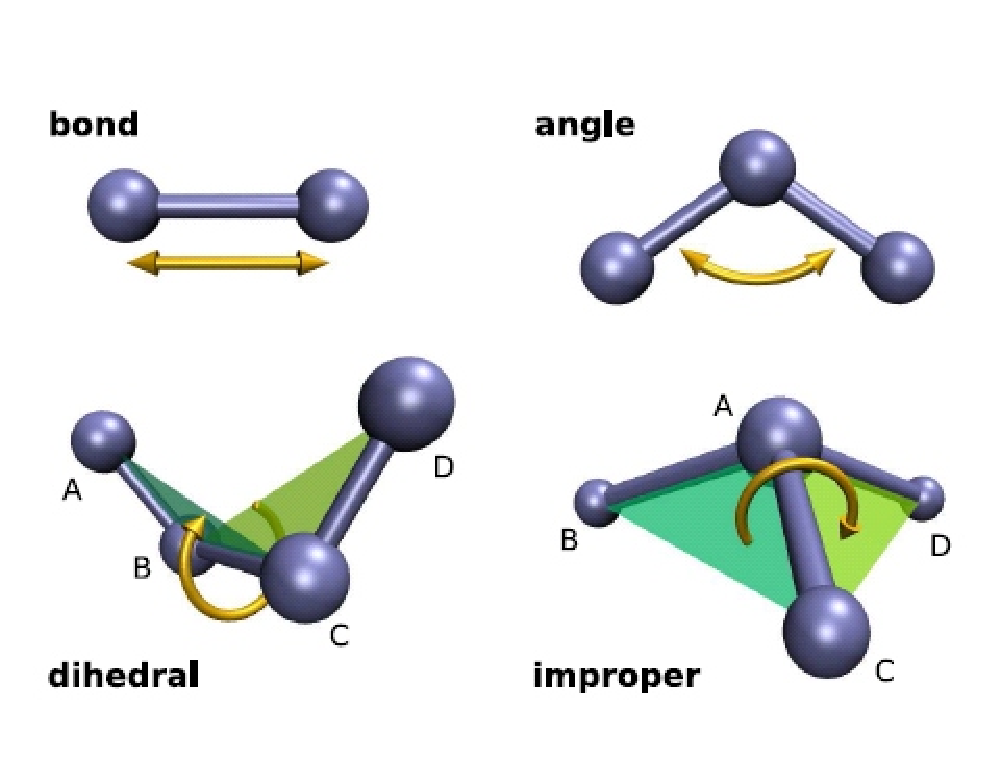
\includegraphics[scale=0.52]{Chapter3/bond1}
\caption[The various bonding between atoms and planes in a molecule.]{The various bonding between atoms and atomic planes in a molecule~\citep{Bergethon1998}.}
\label{bond1}
\end{figure} 

%%%%%%%%%%%%%%%%%%%%%%%%%
{\textbf{Bond Stretching}}:
%%%%%%%%%%%%%%%%%%%%%%%%%
The bond stretching between two bonded atoms \emph{i} and \emph{j} is represented by harmonic potential,
\begin{equation}
{\rm U}_{\rm b}(r_{ij}) =\frac{1}{2}\;k_{ij}^{\rm b}\;(r_{ij} - b_{ij})^2 
\end{equation}
where $b_{ij}$ is the bond length between two atoms and $k_{ij}^{\rm b}$ is the force constant.
%\begin{figure}[h!]
%\centering
%\includegraphics[scale=0.3]{Chapter3/bond}
%\caption{Figure at left represents the schematic diagram of Bond stretching and that at the right is its harmonic potential \cite{Gromacs-manual}.}
%\label{bond}
%\end{figure}

%%%%%%%%%%%%%%%%%%%%%%%%%
{\textbf{Bond-angle vibration}}:
%%%%%%%%%%%%%%%%%%%%%%%%% 
The change in angle between three consecutive bonded atoms (say \emph{i, j, k}) from its equilibrium value causes vibrational motion and this type of vibration is defined by angular harmonic potential. Mathematically, the expression can be written as
\begin{equation}
{\rm U}_{\rm angle}(\Theta_{ijk}) = \frac{1}{2} k_{ijk}^{\Theta}(\Theta_{ijk}- \Theta^0_{ijk})^2.
\label{vibration}
\end{equation}
Here $k^\Theta_{ijk}$ and $\Theta^0_{ijk}$ are the angular force constant and equilibrium bond angle respectively. Since the both, bond stretching and bond-angle vibration, are represented by harmonic potential their curvature seems to be similar. 

%%%%%%%%%%%%%%%%%%%%%%%%%
{\bf Proper dihedral}: 
%%%%%%%%%%%%%%%%%%%%%%%%%
Dihedral angle is based on four-body interactions. Proper dihedral is the angle between two planes made up of four consecutive atoms which constrain the rotation around a bond. In Figure ~\ref{bond1}, two planes are formed by A-B-C and B-C-D. The periodic dihedral potential can be written as, in the form of equation~\ref{proper},
\begin{equation}\label{proper}
{\rm U}_{\rm dihed} = k_{\phi} (1 + \cos(n\phi - \phi_s),
\end{equation}
%%%%%%%%%%%%%%%%%%
where $k_{\phi}$ is force constant, $n$ is multiplicity number, $\phi$ is proper dihedral angle and $\phi_s$ is the angle at which the potential attains its minimum value. The multiplicity ($n$) represents the number of minima when bond is rotated through $2\pi$. 

{\bf Improper dihedral}: Improper dihedral potential forces atoms to remain in a plane or to prevent from transition to its mirror image. Improper dihedral is also the angle between two planes formed by ABC and ACD (Figure \ref{bond1}), however, the atom A remains at the center rather than end of the one of planes in proper dihedral. The harmonic form of improper potential can be represented as,  
%%%%%%%%%%%%%%
\begin{equation}
{\rm U}_{\rm impr} = \frac{1}{2} k_\xi (\xi - \xi_{0})^2 
\label{improper}
\end{equation}
%%%%%%%%%%%%%%%%%
where $k_\xi $ is force constant, $\xi$ is improper dihedral angle and $ \xi_0 $ is equilibrium improper dihedral angle. 

{\textbf{Non- Bonded Interaction}}: Beside the bonded interactions, there are few non-bonded interactions in between the particles. Two of the main non-bonded type are Coulomb and van der Waals (vdW) interactions. In case of non-polar molecules like methane and closed shell atoms like Ar, Kr etc, usually the coulomb interaction is not present. In such a situation, potential energy of a systems is composed of short-ranged repulsive term because of overlapping electron clouds and long-ranged attractive term because of the vdW interactions. The most popular potential which incorporates these terms is called Lennard-Jones (LJ) potential \citep{Kittel2005}. LJ potential is also known as 12-6 potential and represented by,
\begin{equation}
U_{\text{LJ}}(r_{ij}) = 4\epsilon_{ij}\left[\left(\frac{\sigma_{ij}}{r_{ij}}\right)^{12} - \left(\frac{\sigma_{ij}}{r_{ij}}\right)^6\right].
\label{LJI}
\end{equation}
In equation (\ref{LJI}), $\sigma$ and $\epsilon$ are the Lennard-Jones constant, which are usually chosen via empirical methods \citep{Ercolessi1997}. In GROMACS package, these constants are already available for many atoms/systems for further applications. For the structures conducted in the present work, we have chosen force-field parameters from GROMACS itself. 

\begin{figure}[h!]
\centering
\includegraphics[scale=0.4]{Chapter3/Lennard-Jones.eps}
\caption[Lennard-Jones potential for methane dimer.]{Lennard-Jones potential for methane dimer. Data are taken from the GROMOS force field parameters. The symbols $\sigma$ and $\epsilon$ represent the repulsive region and the minimum potential at equilibrium state, respectively.}
\label{lennard}
\end{figure}

When two atoms are brought very close to each other, their electron cloud starts overlapping and causes 
partial promotion of electrons to unoccupied higher energy orbitals~\citep{Kittel2005}. Hence the energy of the system increases, and the interaction becomes repulsive. This phenomenon is described by Pauli-exclusion principle. In equation \ref{LJI}, the repulsive term is represented by the first term $({1}/{r_{ij}})^{12}$ which is obviously dominant at short distances. The second term $({1}/{r_{ij}})^6$, on the other hand, constitutes the attractive part and is dominant at large distances. As we discussed above, this is because of vdW interactions which are originated due to interactions in between electric-dipoles. The vdW interactions are the non-local type of interactions and are the consequences of three different contributions. The contributions from the interactions in between polar molecules or permanent dipoles are referred as Keesom interactions. On the other hand, the vdw interactions in between permanent dipoles and induced dipoles are related to Debye interactions~\citep{Stone1996, Ulman2014}. The most common type of non-local interactions, originated from instantaneous dipole and induced-dipole interactions where the fluctuation of electron density at one region induces dipole into another region of the system, are called London dispersion interactions~\citep{Klime2012}. The London dispersion interactions (proportional to $(1/r_{ij})^6$) is incorporated LJ potential. Although vdW is a weak and long-ranged potential, it is important in the systems with spherical valence shells (where other dominant interactions are absent)~\citep{Leach2001}.

The LJ potential can also be expressed in new parameters, (${C_{ij}}^{(12)}$ and ${C_{ij}}^{(6)}$) 
with ${C_{ij}}^{(12)}= 4\epsilon_{ij} \sigma_{ij}^{12}$ and ${C_{ij}}^{(6)} = 4\epsilon_{ij} \sigma_{ij}^6$. 
Hence equation \ref{LJI} becomes 
\begin{equation}\label{LJ}
U_{\text{LJ}}(r_{ij}) = \left[\frac{C_{ij}^{(12)}}{r_{ij}^{12} } - \frac{C_{ij}^{(6)}}{r_{ij}^6 }\right]
\end{equation}
One can use proper combination rules to calculate the parameters of molecules with different values of atomic LJ constants~ \citep{Gromacs-manual}.

%%%%%%%%%%%%%%%%%%%%%%%%%
{\textbf{Coulomb Interaction}}: 
%%%%%%%%%%%%%%%%%%%%%%%%%
Coulomb interaction may exist in between the point charges of same or different molecules. For any two
point charges $q_i$ and $q_j$ separated by distance $r_{ij}$, the coulomb term can be expressed as:
\begin{equation}
\textrm{{U}}_{\rm coulomb} = \frac{q_iq_j}{4\pi\epsilon\epsilon_or_{ij}}
\label{Coulomb}
\end{equation}
In equation (\ref{Coulomb}), $\epsilon$ and  $\epsilon_\circ$ represent the dielectric constant and the permittivity of free space, respectively. Coulomb potential has very important role in case of ionic system, and sometimes may exist in non-ionic systems when electron density in valence shells shifts due to unequal values of electronegativity of atoms.

\begin{sloppypar}
{\textbf{Periodic Boundary Conditions (PBCs)}}: Particles at/near to the surface feel different forces than that of the particles deep inside the surface(boundary) \citep{Allen1989}. Ideal infinite-systems have no surface atoms, however, the real systems are different from this hypothesis. For an example, in case of 1000 atoms in a cubical box (arranged by $10\times10\times10$), more than 488 atoms appear at the surface of the cube \citep{Allen1989}. In larger (macroscopic) systems, only a small fraction of atoms are close enough to the surface of the container to realize the surface effects (an effect due to presence of surface or wall of the container which provide rigid boundary for atoms while trying to escape during the simulation). 
\end{sloppypar}

The system-size of usual molecular dynamics is limited to few thousands of atoms because of complexity in structure and computational limitations. The smaller systems are dominated by surface effects, and one of the 
easiest ways to minimize the surface effect is to consider the periodic boundary condition where the system is surrounded by the copies of its images \citep{Frenkel2002}. It means the box containing N number of atoms (to be simulated) is assumed to be a primitive cell which is propagated through out the space to construct an infinite system. Hence the boundary of the central box has been removed and the particles feel no surface effects. During the course of simulation, when one particle leaves the box from one side, its nearby image enters into the box from another side keeping the number density of the system fixed~\citep{Hansen2006}. 
%%%%%%%%%%%%%%%%%%%%
\begin{figure}[h!]
\centering
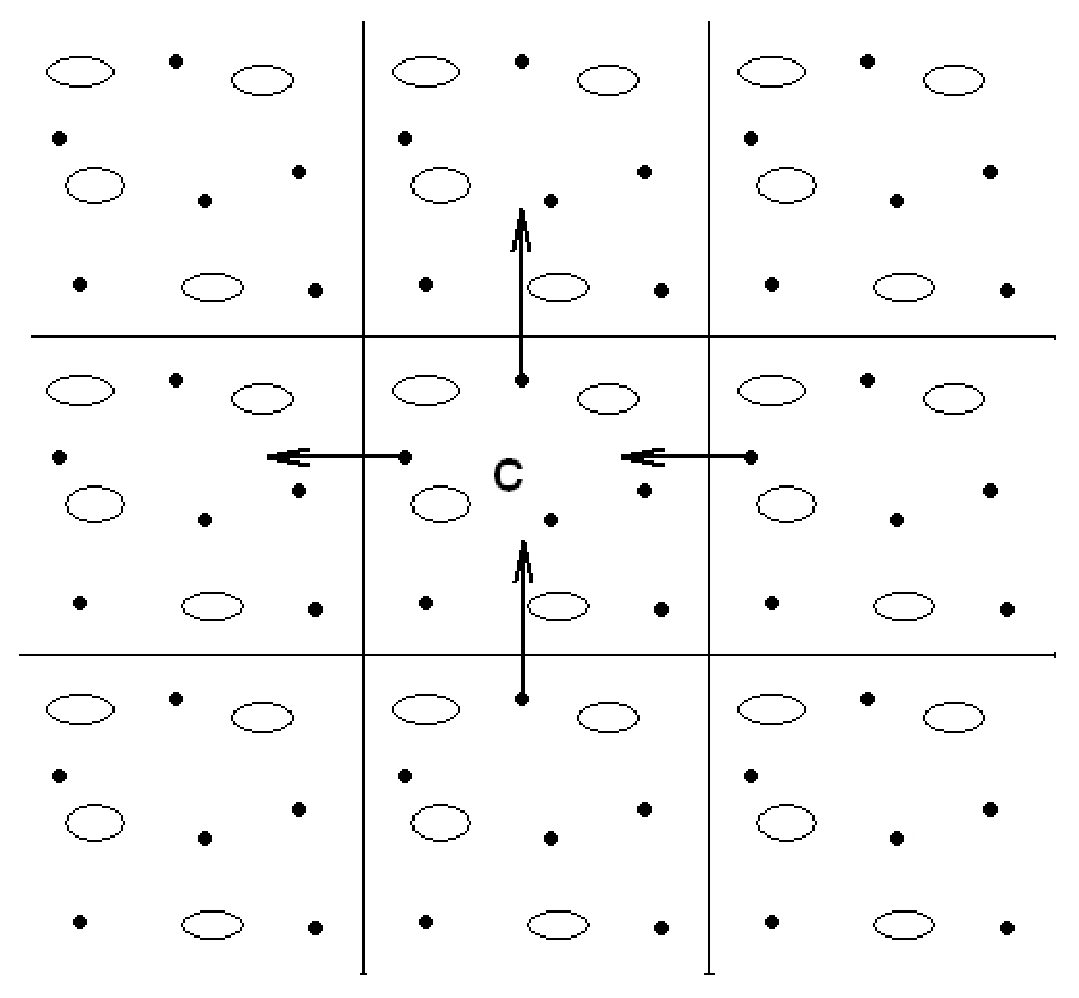
\includegraphics[scale=0.52]{Chapter3/pbc.eps}
\caption[Schematic representation of periodic boundary conditions.]{Schematic representation of periodic boundary conditions \citep{Gromacs-manual}.}
\label{pbc}
\end{figure}
%%%%%%%%%%%%%%%%%
Another consequence of PBC is {\it minimum image criterion} which is applicable to limit the interaction between the particles. That is among $N$ number of particles, each atom interacts with the closest images of other $N - 1$ particles and ignores all remaining images \citep{Allen1989}. Since the potential is considered through pairwise addition of the interactions, the total potential involves $N(N - 1)/2$ terms, which is still high and can be reduced further ( for short range interactions) by using spherical cut-off. To avoid the images from double counting, the value of cutoff (say $R_{\text{c}}$) should not be greater than half of the box size \citep{Ercolessi1997}. For long range interactions (like for ionic systems), however, truncation of potential at small $R_{\text{c}}$ can not include the interactions at longer distances and causes a serious problem. This problem can be minimized by using the method of Ewald, where short-range potential is summed in real space with appropriate truncation, and the long-range summation is taken over the reciprocal lattice vectors \citep{Hansen2006}.

Although the size effect is minimized by using PBC, it is not the absolute solution. Its magnitude depends up on the kind of the system and the properties of interest. One can check varying size samples to estimate the size effect and possible error due to chosen size~\citep{Poudyal2014}. 
%%%%%%%%%%%%%%%%%%%%%%%%%
\subsection{Initialization} \label{Initial-MD}
%%%%%%%%%%%%%%%%%%%%%%%%%
\begin{sloppypar}
Initialization is the step to assign the initial co-ordinates and velocities which should be compatible to the structures. One has to exclude the overlap of atomic cores while choosing positions in this stage. The velocities are attributed by using Maxwell-Boltzmann distribution and scaled to adjust the mean kinetic energy to the desired values \citep{Gromacs-manual}. The relationship of velocity with temperature in thermal equilibrium is given by \citep{Frenkel2002},
\end{sloppypar}
\vspace{-25pt}
\begin{equation}
\langle v_\alpha^2 \rangle = \frac{k_{\text{B}} T}{m}.
\end{equation}
Here $v_\alpha$ is the $\alpha(x,y,z)$ component of the velocity, $m$ is the mass of a given particle, $T$ is the temperature and $k_{\rm B}$ is Boltzmann's constant. 
%%%%%%%%%%%%%%%%%%%%%%%%%
\subsection{Force Calculation}
%%%%%%%%%%%%%%%%%%%%%%%%%
\begin{sloppypar}
The main step of MD simulations after {\it initialization} of a system, is the calculation of forces acting on each of the particles. This process includes the estimation of forces on a particle $i$ due to all its neighbors \citep{Ercolessi1997}. By using the relation of potential, which is pairwise addition of interacting particles ${\rm U}(r_i)$, the force can be calculated by
\begin{equation}
\mathbf{F_i} = -\nabla_i\textrm{U}(\mathbf{r}_i).
\end{equation}
Calculation of forces should include all the interacting particles within the range of defined cutoff and excludes all the remaining ones. 
The procedure follows the {\it minimum image convention} where particle $i$ interacts with the nearest image of $j$ \citep{Frenkel2002, Ercolessi1997}. \end{sloppypar}

\begin{figure}[h!]
\centering 
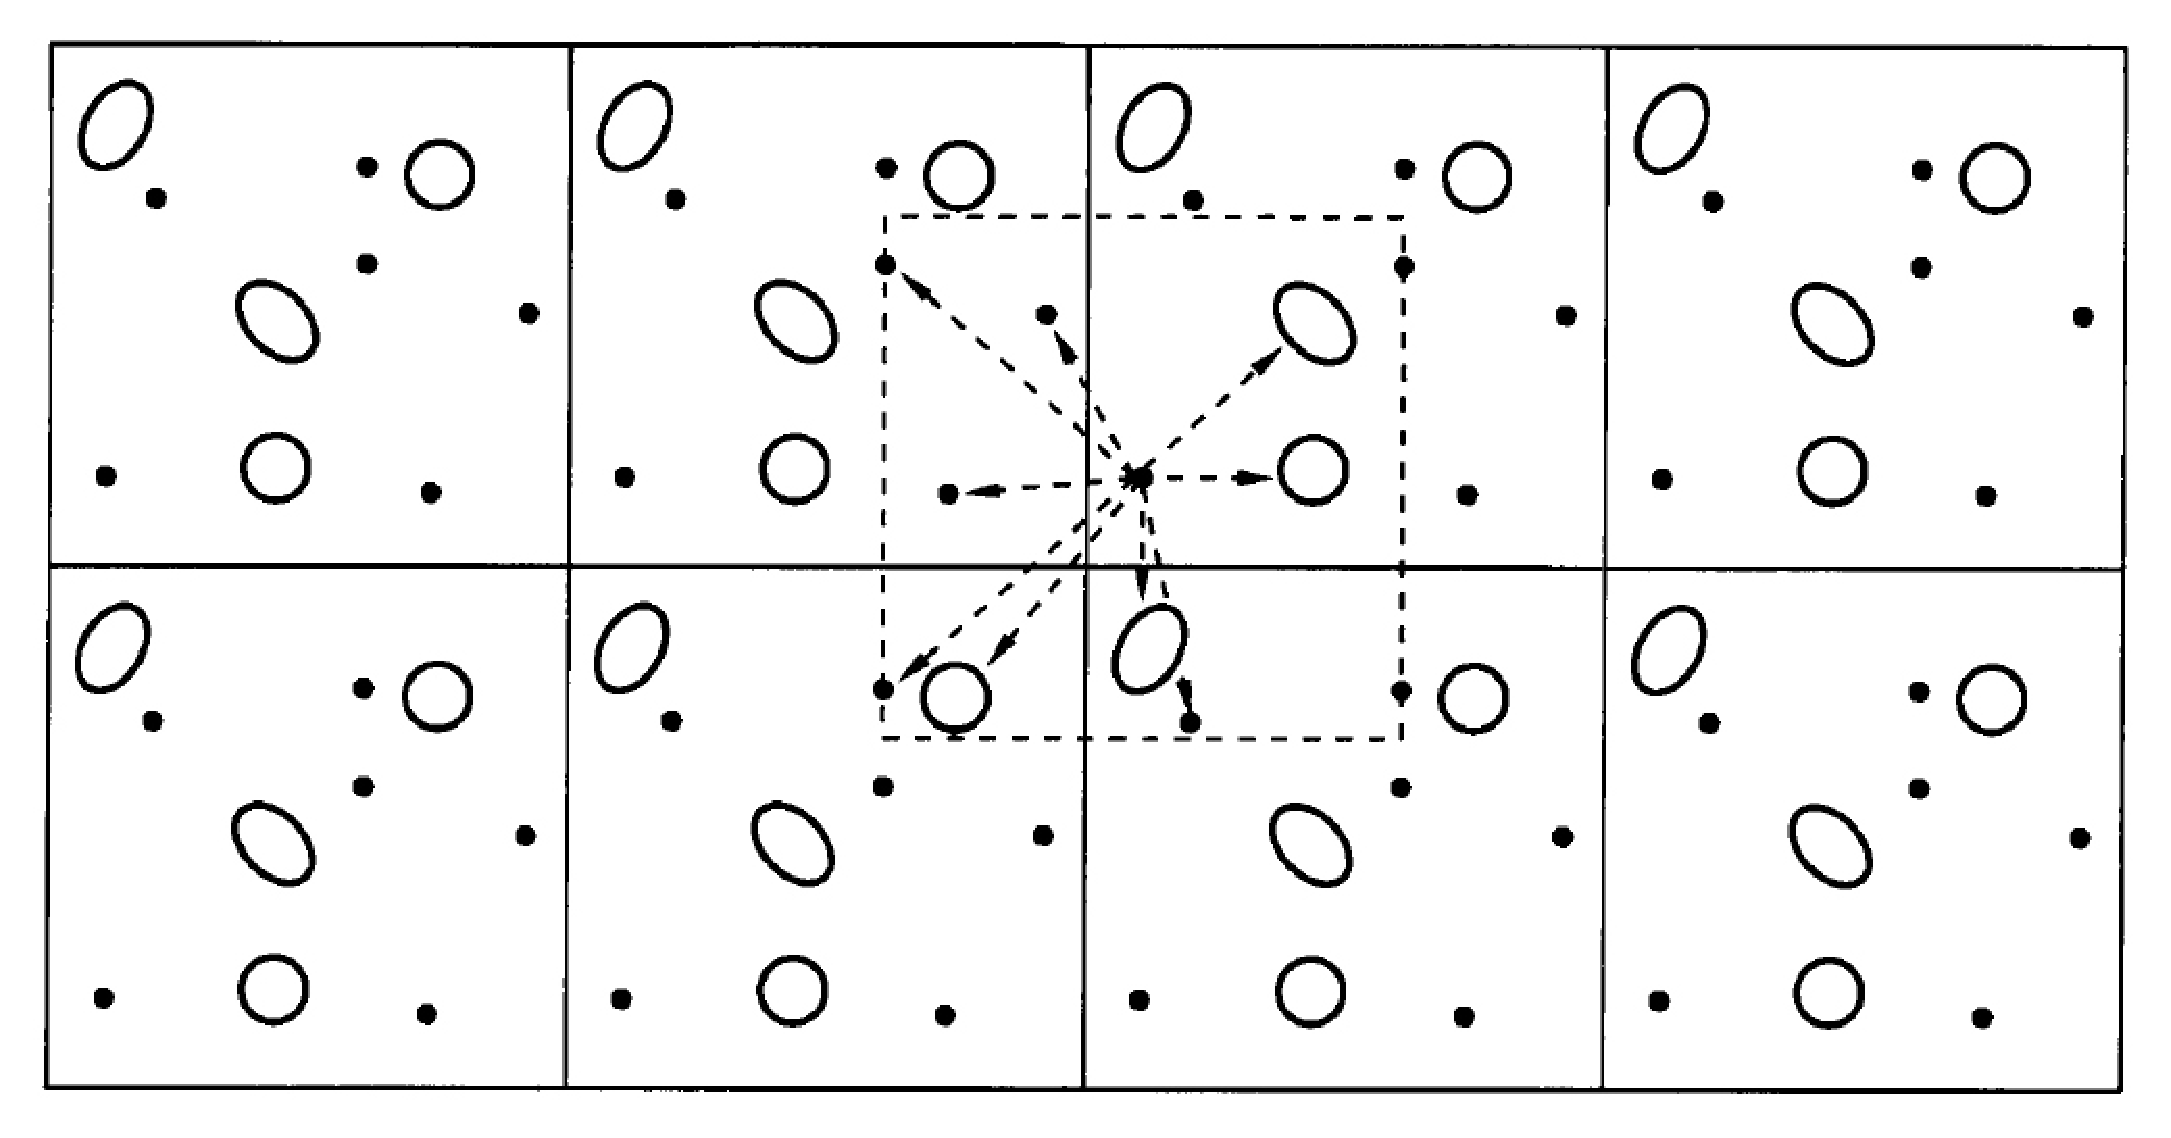
\includegraphics[scale=0.38]{Chapter3/cutoff.eps}
\label{cutoff}
\caption[Cut-off and near-image convention for periodic boundary condition. ]{Use of cut-off and near-image convention for periodic boundary condition \citep{Frenkel2002}.}
\end{figure}

The value of cutoff ${\rm R}_{\text{c}}$ can not be large enough due the limitations on the size of the simulating box 
(${\rm R}_{\text{c}}$ should not be greater than half of the box-size). For long range interactions, however, the interaction beyond ${\rm R}_{\text{c}}$ could be significant and needs correction. One of corrections is based on mean field approximation where the field beyond ${\rm R}_{\text{c}}$ is constant \citep{Thapa2013}. Another usual method for the correction includes Ewald summation in which all interactions between the particle {\it i} in the central cell and its (unit cells) replica surrounding the central one are integrated~\citep{Gromacs-manual}.
%%%%%%%%%%%%%%%%%%%%%%%%%
\subsection{Integration of Equation of Motion}
%%%%%%%%%%%%%%%%%%%%%%%%%
The calculations of new coordinates for position and components of velocities of particles by using their initial (known) information is related to the solution of equations of motion. The forces are position dependent through potentials, and mathematical algorithms are able to predict the new coordinates by using the available information. Hence the phase space coordinates generate their trajectories. There are many methods to trace these trajectories, and the methods with higher precision with the least possible computational cost are supposed to be the most preferred ones. The precision and computational cost are contradictory for a simulation, and requires compromise in between their perfect conditions\citep{Allen1989}. In case of MD simulations, the length of time step is one of the major determining factors for computational cost (the higher the time step, 
the lesser the computational cost) and accuracy (the smaller the time step, the higher the accuracy).
%%%%%%%%%%%%%%%%%%%%%%%%%
\subsection{Verlet Algorithm}
%%%%%%%%%%%%%%%%%%%%%%%%%
\begin{sloppypar}
One of the popular methods for integrating the equations of motion is Verlet algorithm where the positions $\textbf{r}(t)$, and
accelerations $\textbf{a}(t)$ are found from the previous steps~\citep{Frenkel2002}. The relations for Verlet algorithm are based on Taylor series expansion, by using which for the time step $\delta t$ we get 
\end{sloppypar}
\vspace{-20pt}
\begin{align}
\textbf{r}(t+\delta t) & = \textbf{r}(t) + \textbf{v}(t) \delta t + \frac{\textbf{F}(t)}{2 m} \delta t^2 + \frac{\delta t^3}{3!} \frac{d^3 r}{d t^3} + O(\delta t^4) \label{ver1} \\
\textbf{r}(t-\delta t) & = \textbf{r}(t) - \textbf{v}(t) \delta t + \frac{\textbf{F}(t)}{2 m} \delta t^2 - \frac{\delta t^3}{3!} \frac{d^3 r}{d t^3} + O(\delta t^4) \label{ver2}
\end{align}
Now adding equations (\ref{ver1}) and (\ref{ver2}) we get 
\begin{align}
\textbf{r}(t+\delta t) + \textbf{r}(t-\delta t) = 2 \textbf{r}(t) + \frac{\textbf{F}(t)}{m} \delta t^2 + O(\delta t^4) \\
\textbf{r}(t+\delta t) = 2 \textbf{r}(t)-\textbf{r}(t-\delta t) + \frac{\textbf{F}(t)}{m} \delta t^2 + O(\delta t^4)
\label{ver3}
\end{align}
Equation (\ref{ver3}) shows that error in position is in the order of $\delta t^4$. Velocities are importat to estimate the kinetic energy (however are absent in position trajectories), and can be obtained by using equations
(\ref{ver2}) and (\ref{ver1}). 
\begin{align}
& \textbf{r}(t+\delta t) - \textbf{r}(t-\delta t) = 2 \textbf{v}(t) \delta t + O(\delta t^3) \\
\label{verlv}
& \textbf{v}(t) = \frac{\textbf{r}(t+\delta t) -\textbf{r}(t-\delta t)}{2 \delta t} - O(\delta t^2) 
\end{align}
Since the error of velocity is in the order of $\delta t^2$ (comparing to $\delta t^4$ in positions), accuracy 
is expected to be lower in velocity. Furthermore, velocity and positions could not be calculated simultaneously, 
that is velocity at time t needs the coordinates at $t+\delta t$. 

\subsection{Leap frog Algorithm}
Leap frog algorithm  is an equivalent scheme to Verlet algorithm. It is named for half-integer time steps of velocities with respect to positions (and acceleration), and uses these velocities to compute the new positions. 
It means that velocities leap over the position coordinates to give the next mid step values (Figure~\ref{leap_frog}) ~\citep{Frenkel2002}. If $(t-\delta t/2)$ and $(t+\delta t/2)$ are the mid-integer time steps, the corresponding velocities are defined by
%%%%%%%%%%%%%%%%%%%%%
\begin{equation}
\textbf{v}\left(t-\frac{\delta t}{2}\right) \equiv \frac{\textbf{r}(t)-\textbf{r}(t-\delta t)}{\delta t}
\label{v-minus}
\end{equation}
and \begin{equation}
\textbf{v}\left(t+\frac{\delta t}{2}\right) \equiv \frac{\textbf{r}(t + \delta t) - \textbf{r}(t)}{\delta t}\,.
\label{v-plus}
\end{equation}
%%%%%%%%%%%%%%%%%%%%
The new positions can be calculated from  the old positions and velocities. 
\begin{equation}
\textbf{r}(t+\delta t) = \textbf{r}(t) + \textbf{v}\left(t+\frac{\delta t}{2}\right) \delta t  
\end{equation}
%%%%%%%%%%%%%%%%%%
By using the Taylor series expansion on velocity about $t$, we get the Verlet type relations as
\begin{equation}
\textbf{v}\left(t+\frac{\delta t}{2}\right) = \textbf{v}(t) + \frac{\textbf{F}(t)}{2 m} \delta t\, .
\end{equation}
Again,
\begin{equation}
\textbf{v}\left(t-\frac{\delta t}{2}\right)= \textbf{v}(t) - \frac{\textbf{F}(t)}{2 m} \delta t\, .
\end{equation}
Solving the above two equations we get
\begin{equation}\label{leap_v}
\textbf{v}\left(t+\frac{\delta t}{2}\right) = \textbf{v}\left(t-\frac{\delta t}{2}\right) + \frac{\textbf{F}(t)}{m} \delta t\, .
\end{equation}
Since the velocities and positions are defined at different time, potential energy and kinetic energies can not be defined simultaneously. It means the total energy can not be calculated directly from the above equations. However, the trajectories for the position and velocities are similar~\citep{Ercolessi1997, Bergethon1998}. The schematic representation of Leap frog algorithm is shown in Figure \ref{leap_frog}.

\begin{figure}[h!]
\centering
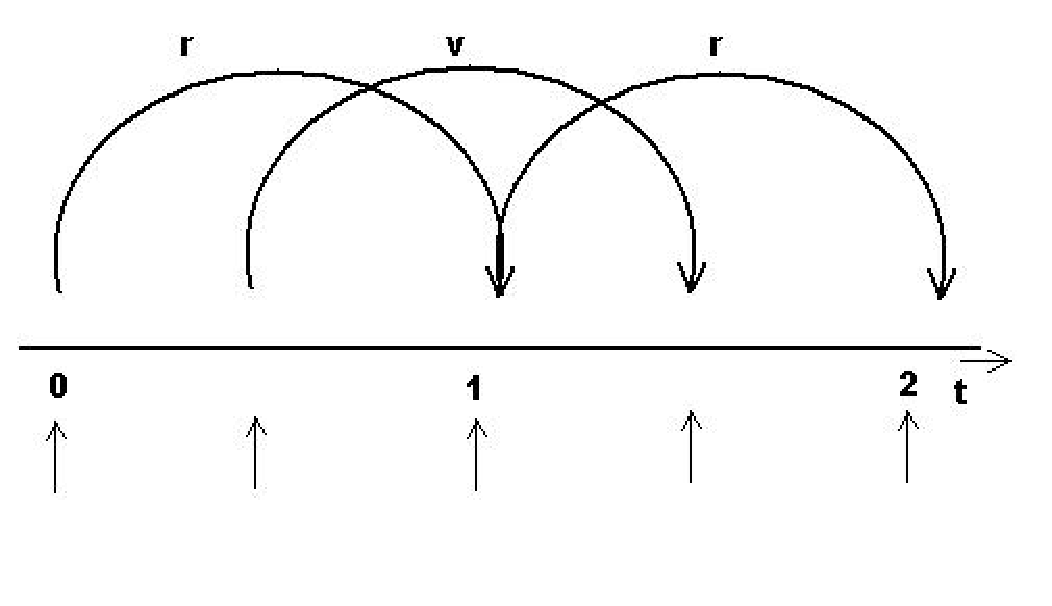
\includegraphics[scale=0.40]{Chapter3/leapfrog.eps}
\caption[Schematic representation of leap-frog algorithm. ]{Schematic representation of leap-frog algorithm \citep{Frenkel2002}.}
\label{leap_frog}
\end{figure}
Time reversibility is one of the major applications of leapfrog integration. It means integration for n steps forward, and then $n$ steps backwards bring the system at the starting (same) position~\citep{Allen1989}. 
The velocities at current time {\it t} can also be calculated via indirect method (by using equations \ref{v-minus} and \ref{v-plus}), 
\begin{equation}
\textbf{v}(t) = \frac{1}{2} \left(\textbf{v}\left(t + \frac{1}{2} \delta t\right) + \textbf{v} \left(t - \frac{1}{2} \delta t\right)\right)\,.
\end{equation}
\subsection{Constraint Dynamics}
The non-polar spherical atoms can be treated with the LJ potential which used to be the obvious choices in early 
MD simulations \citep{Harp1968, Harp1970}. In molecular systems, however, the fundamental particles interact with intra- and intermolecular forces which are accounted by bond vibrations and changes in relative orientation etc. Some of these vibrations are very fast and require extremely short time step. This complexity in simulations can be replaced by constraint dynamics where the intra-molecular bonds and angles are supposed to be fixed. The magnitude of vibrations are small comparing to their molecular dimensions, and this assumption is near to the reality. For such a purpose, we need a constraint to force the system into required rigidities \citep{Leach2001}. SHAKE and LINCS are two popular constraints available in GROMACS package.  In the present work, we have used SHAKE as constraint algorithm where a set of unconstrained co-ordinates are changed to another set that are constrained with distances~\citep{Gromacs-manual}.
%%%%%%%%%%%%%%%%%%%%%%%%%
\section{ Statistical Ensembles in Molecular Dynamics}
%%%%%%%%%%%%%%%%%%%%%%%%%
The dynamical state of any system (having $N$ number of particles) is defined by $3N$ position and $3N$ momentum coordinates. A set of these $6N$ variables define a micro-state in $6N$ dimensional phase space which is called phase point. We introduce {\it ensemble} to explain the probability distribution of the microscopically defined states of a system in terms of imaginary collections of the system. Each of these collections is the replica of real systems with same macroscopic properties. The concept of such ensembles realize the physical observables in terms of their average values~\citep{Pathria1996}.

Depending up on the variables kept fixed in the systems, ensembles are classified as microcanonical (NVE), canonical (NVT), isothermal-isobaric (NPT) and grandcanonical ($\mu$VT) ensembles. The symbols refer to the number of particles (N), volume (V), energy (E), pressure (P) and temperature (T) and the combination of these variables define the type of ensemble. Constant temperature, and constant pressure experiments respectively, are relevant to NVT and NPT ensembles. Microcanonical (NVE) ensembles are very common in MD simulations. Upon 
having enough lapse of time in MD simulations time average of desired properties like: total energy, can be replaced by ensemble averages (average property of large number of replications of systems at a time) which simplifies calculating the properties of interest. Such a condition where the time average of an observable in a system is equivalent to the ensemble average, is called ergodic \citep{Leach2001}. 

In MD simulations, pressure and temperature vary a lot. To fix them, some regulatory mechanisms are required \citep{Leach2001}. For the purpose of controlling temperature (T) and pressure (P), we have different coupling systems, and some of them are described in the following paragraphs. 
%%%%%%%%%%%%%%%%%%%%%%%%%
\subsection{Temperature Calculation and Control} \label{thermostat}
%%%%%%%%%%%%%%%%%%%%%%%%%
The initial particle velocities in a system are defined by Maxwell-Boltzmann distribution as described in section~\ref{Initial-MD}. During the course of simulation, however, the velocity distribution changes to new values. Since the velocities are correlated with the kinetic temperature of the system, they need to be rescaled according to the target temperature which is the requirement for constant temperature ensembles. The ensembles with constant temperature are either NVT or NPT. The constant temperature condition is also the fundamental requirement for correct ensemble averages to study the properties of the system as a function of temperature like folding and unfolding  of proteins \citep{Leach2001}. The temperature-controlled simulations are also important in order to systematically increase or decrease the temperature of the system like for simulated annealing. The correct temperature, within reasonable fluctuations, is maintained by using different types of temperature-control mechanisms like rescaling the velocities or by external heat baths (thermostats) \citep{Frenkel2002}. The choice of the thermostat depends on the nature of system and the properties of interest. Berendsen thermostat is useful for the cases of weak coupling scheme \citep{Berendsen1984} and the extended-ensemble approach is attained by Nose-Hoover thermostat \citep{Nose1984, Hoover1985}. We have used velocity-rescale (v-rescale) type of thermostat for such purpose. Velocity-rescale thermostat is basically identical with the Berendsen thermostat except few extra terms which ensure a correct kinetic energy distribution~\citep{Gromacs-manual}.

Rescaling velocities to control the temperature are related through the time average kinetic energy of the system, $\left\langle \text{K.E.} \right\rangle = \frac{3}{2} k_{\rm B}T$, with some rescaling factor, $\lambda = [ {\rm T}_{\rm new}/{\rm T}(t) )^{1/2}]$. Here ${\rm T}_{\rm new} $ and $ {\rm T}(t) $ are new temperature after rescaling velocities and temperature at time $ t $ respectively.

Heat baths, on the other hand, exchange heat with the system to attain the target temperature.  
\begin{equation}\label{thermo}
\frac{d{\rm T}(t)}{dt}  =  \frac{1}{\tau} ( {\rm T}_{\rm bath} - {\rm T}(t)),
\end{equation}
where $\tau$, ${\rm T}_{\rm bath}$ and T($t$) represent the coupling constant, target (bath) temperature and the temperature at time $t$ respectively.

In the microcanonical ensemble (constant NVE), temperature is defined by making use of the equipartition principle which states that the average kinetic energy per degree of freedom is $\frac{k_{\rm B}{\rm T}}{2}$. The instantaneous temperature in such a system becomes  
\begin{equation}
{\rm T}(t) = \frac{2}{(3N - N_{\text{c}})k_{\rm B}}\sum_j^N\frac{1}{2}m_iv_i^2(t)
\end{equation}
Here ${N}$ and ${N}_{\text{c}}$ represent the number of particles and number of constraints on the system, respectively. Similarly, $m_i$ and $k_{\rm B}$ represent mass of the $i^{\rm th}$ particle and Boltzmann's constant respectively.
%%%%%%%%%%%%%%%%%%%%%%%%%
\subsection{Pressure calculation and control}
%%%%%%%%%%%%%%%%%%%%%%%%%
As similar to the constant temperature, constant pressure simulations are important in many practical cases. The experiments at constant pressure are very common and computational work at similar condition is relevant for the purpose of estimation and comparison with the experiments. At fixed temperature (see subsection~\ref{thermostat}), NPT ensemble is characterized by constant pressure and number of particles. In practice, constant pressure simulations are  important to study the system-properties as a function of pressure such as pressure induced phase transitions \citep{Leach2001}. 

Since the constant pressure is usually maintained by changing volume, the observation of fluctuations in volume are important. NPT system is related to isothermal compressibility with the relation
\begin{equation}
\kappa  = - \frac{1}{V} \frac{{\partial}{\rm V}}{{\partial} {\rm P}} .
\end{equation}
This indicates that the easily compressible substance has larger changes/fluctuations in volume, comparing to the incompressible substances. In the reverse way, less compressible substance has larger fluctuations in pressure at constant volume. As similar to the control in temperature, there are various schemes to control pressure. They could be either by scaling the volume or by using pressure bath (barostats) \citep{Gromacs-manual}, 
\begin{equation}
\frac{\d{\rm P}(t)}{\d t}  =  \frac{1}{\tau_p} ( {\rm P}_{\rm bath} - {\rm P}(t)). 
\label{baro}
\end{equation}
\begin{sloppypar}
In the equation (\ref{baro}), $\tau _p$, ${\rm P}_{\rm bath}$ and P($t$) represent the coupling constant, target (bath) pressure and the pressure at time $t$ respectively. Pressure is felt by the momentum carried out by the particles while they cross the boundary and the force of interaction in between the particles at different surfaces. There are different types of barostats to control the pressure inside a simulation box, which are described in available literature~\citep{Parrinello1981, Melchionna1993, Andersen1980}. In the present work, 
we have used Parrinello-Rahman type of barostat for such a purpose. In Parrinello-Rahman Barostat, box-vectors follow an equation of motion where the equation of motion of the particles are also changeable. This type of barostat can also be applied in varying shapes of simulation cells~\citep{Parrinello1981}.
\end{sloppypar}
%%%%%%%%%%%%%%%%%%%%%%%%%
\subsection{Umbrella Sampling}
%%%%%%%%%%%%%%%%%%%%%%%%%
Thermally favorable microstates of a system are more frequently visited by the simulation trajectories in normal 
computational techniques (Boltzmann-like weights). There are some states, which are hindered by energy barriers, are either rarely sampled or not visited at all~\citep{Allen1989}. For a number of properties, such as free energy difference which is especially important in biological systems \citep{Kastner2011}, are difficult to calculate via such direct simulation techniques due to the requirement of very high computational resources and length of time. However, few techniques with non-Boltzmann sampling are available to weight different energy states differently which encourages the system to visit the regions of the phase space not usually sampled by the direct approach.  The usual techniques in use are umbrella sampling, thermodynamic integration, slow growth, steered MD etc~\citep{Frenkel2002, Kastner2011}. {\it Umbrella Sampling} which literally means bridging the gap (umbrella) between two or more states, is an enhanced molecular dynamics where the potential is biased along the reaction coordinates and shifts a system from one thermodynamic state to another. Any type of potential, in principle, can be used as biasing potential, however harmonic potential is one of the frequently used schemes to overcome the effect of energy barrier in Boltzmann distribution. The algorithm introduces different windows against the reaction co-ordinates to sample the system throughout the regions of its energy landscape. The information from the different windows are then combined via appropriate method to calculate the required parameter. In the present work, we have used weighted histogram analysis method (WHAM) for such a purpose \citep{Kumar1992}. WHAM is one of the popular methods to extract PMF which is useful to find the free energy difference against the reaction coordinates. The process uses the information of output files obtained from umbrella sampling simulations. 
 
 \begin{sloppypar} 
The technique of umbrella sampling was first suggested in 1977 by \citep{Torrie1977a}. The later developments were introduced to study the liquid mixture \citep{Torrie1977b}, to calculate the excess surface energy of a water model \citep{Lee1980} and chemical potential of a particle in a fluid \citep{Shing1981}. We use the technique of potential of mean force (PMF), defined as the potential that is obtained by integrating the mean force from ensemble of configurations, by using the method of umbrella sampling simulations~\citep{Gromacs-manual}. 
 \end{sloppypar}
  
{\bf Potential of mean force}: Solute-solute interactions is the primary concern of the present work. However, the average solvent-effects is important factor to be incorporated in many fields of research. Potential of mean force is an approach to observe changes in free energy with respect to some particular coordinates like separation between the solute particles \citep{Leach2001}. The method of PMF enables to study the modulating effect of solvents on the dynamics of the system through collision and viscus drag force. 
 
PMF is the free energy surface along the chosen co-ordinates. The highest energy point of the surface thus represents the transition state of different phenomenon. Mathematically, PMF can be obtained by using the information of radial distribution function (RDF). Hence the Helmholtz free energy can obtained from PMF with the expression,  
\begin{equation}\label{Helmholtz}
{\rm F}(r) = - k_{\rm B}{\rm T} \ln[g(r)] + {\rm constant}.
\end{equation}
With relation \ref{Helmholtz}, small change in free energy causes a change in $g(r)$ from its most likely value which are not sampled by usual MD simulations. The method of biased simulations like umbrella sampling becomes relevant in such cases. 
 
The usual potential is modified with the addition of some suitable type of potential which helps to sample unfavorable states sufficiently. The biased potential thus becomes, 
\begin{equation}\label{biased}
{\rm V'}(r^N) =   {\rm V}(r^N) + {\rm W}(r^N)
\end{equation}
where ${\rm V}(r^N)$ and ${\rm W}(r^N)$ are the unbiased potential and weighing function. The weighing function is usually quadratic in nature. The 
general expression thus becomes
\begin{equation}\label{quadratic}
{\rm W}(r^N) = k_W (r^N-r_0^N).
\end{equation}
In equation~\ref{quadratic}, $(r^N-r_0^N)$ measures how far the system is from the equilibrium state $r_0^N$. The weighting function $({\rm W}(r^N))$ is large for the configurations which are far from the equilibrium state. The 
resulting distribution is non-Boltzmann type where the Boltzmann distribution for them can be extracted as per method suggested by Torrie and Valleau \citep{Torrie1977a}. For a quantity $A$, the average value is defined as, 
\begin{equation}\label{non-boltzmann}
\langle A \rangle = \frac{ \langle A(r^N) \exp[+W(r^N)/k_{\rm B}T]\rangle _W}{\langle \exp[+W(r^N)]\rangle_W}.
\end{equation}
The average value, based on probability ${\rm P}_W(r^N)$ and determined via modified potential ${\rm V'}(r^N)$, is represented by subscript ($W$). In case of umbrella sampling simulations, a series of appropriate biasing potentials are generally applied with the caution that very large values of biasing for some of the windows may cause controlling the result by a few configurations. Insufficient biasing, on the other hand, is incapable to constrain the system at the target region of the phase space.

The method of simulation for {\it umbrella sampling} is not very different than usual MD. The initial configurations are prepared for a series of reaction coordinates. For an example: when the free energy surface (PMF) for the interactions between two solute molecules in solvent environment is to be determined against the distance between them (as reaction coordinates), a series of windows with varying distance are prepared. The simulating potential is biased with additional harmonic potential (say) for each configuration with appropriate overlapping in between the nearest windows. The biasing potential for each window which aims to constrain the system within certain region of the phase space, can be varied depending upon the nature and range of interactions.

\begin{figure}[h!]
\centering
%\includegraphics[scale=0.40]{Chapter3/Folw_chart_us_next-0.eps}
\includegraphics[scale=0.40]{Chapter3/Flow_chart_umbrella.eps}
\caption{Flow chart representation of umbrella sampling simulations.}
\label{umbrella_flow}
\end{figure}

Flow chart (Figure \ref{umbrella_flow}) shows that the construction of correct topology file is the first step of the simulation process. This can be done by using the coordinate file of the system via proper GROMACS executable (pdb2gmx). The choice of right size of the box and the number of solvent molecules are the next steps of the simulation which need care of nature of interactions and minimum image criteria. According to this convention, the separation between the molecules can not be greater than the half of the box size. In the process of minimization, the system finds its structure and configurations corresponding to local minimum searched by the appropriate algorithm (gradient of potential is zero in such points)~\citep{Gromacs-manual}. Minimization removes the bad contacts caused by the improper position of the atoms and avoids being far from the equilibrium configuration. A series of windows are then generated to run the separate simulations as shown in Figure (\ref{windows}). 

\begin{figure}[h!]
\centering
\includegraphics[scale=0.40]{Chapter3/Windows.eps}
\caption[Schematic representation of a series of windows prepared for umbrella sampling simulations.]{Schematic representation of a series of windows prepared for umbrella sampling simulations. The reaction coordinates are taken as the separation between two atoms (red large and small blue atoms). (Retrieved from: \url{http://www.gromacs.org/@api/deki/files/205/=pmf_tutorial_online.pdf}, dated: June 6, 2016).}
\label{windows}
\end{figure}

The first row in Figure (\ref{windows}) represents the pulling simulation which helps to construct many windows against the reaction co-ordinates (shown in second row with respect to red large atom). The strength of biasing potential and separation between the windows are correlated and taken into care on the ground of adequate overlapping between the nearest windows. {\it Pull code} defines the distance between the center of masses of the interacting molecules or groups and takes care of correlation between the windows~\citep{Gromacs-manual}. Each of the windows are then simulated for the appropriate time step. The biased information thus collected is unbiased and analyzed by different methods. We use WHAM to calculate free energy surfaces, binding energy 
and also the solvent perturbation in solute-solute interactions.
%...............................................................................................
%%%%%%%%%%%%%%%%%%%%%%%%%
\section{Systems under study}
%%%%%%%%%%%%%%%%%%%%%%%%%
In the present work, interactions of methane with other like and unlike atoms are studied in methane hydrates, functionalized graphene and methane dipoles at liquid environments. 
%%%%%%%%%%%%%%%%%%%%%%%%%
\subsection{Methane hydrate} \label{hydrate_system}
%%%%%%%%%%%%%%%%%%%%%%%%%
The methane-rich clathrates are the high pressure compounds and have multiple structures with reference to varying environmental conditions \citep{SloanJr2007}. We have considered methane hydrate III (MH-III) as a sample where four methane molecules (in each unit cell) are encapsulated within the ice channels of eight water molecules~\ref{MH-III-stru}. The initial structure of MH-III was constructed at 10~GPa where the internal coordinates and the lattice parameters were taken from experimental data~\citep{Loveday2001}. Since the authors used X-rays diffraction method to retrieve the experimental data, only the atomic coordinates of the heavier atoms, carbon and oxygen, are available. The positions of hydrogens for the water molecules were chosen to satisfy the ice rules. There are multiple ways to satisfy the ice rule, the structures with vanishing (anti-ferroelectric) and non-vanishing (ferroelectric) dipole moments were considered in the present calculations. The ferroelectric structure was basically assumed at some representative pressures, including extreme and moderate values, for the purpose of checking the effect of structural arrangement on stability/enthalpies. The initial orientations of the methane molecules were fixed arbitrarily and also the effect of different orientations were checked by using three configurations of methane as definition used by Wood et al. ~\citep{Wood2012}. The configurations based on their orientation are defined by Straddle (S), Tripod Towards (TT) and Tripod Away (TA) with reference to a particular direction. All the parameters (lattice and internal) were relaxed at zero temperature and fixed pressure values, from 10~GPa to 300~GPa, in steps of 10~GPa. Pressure was varying in both the directions, increasing from minimum (10 Gpa) towards the maximum (300 GPa) and vice-versa, during the simulations. 
 
\begin{figure}[h!]
\begin{center} 
%\subfigure[Ferroelectric]{\includegraphics[width= 0.3\textheight]{Chapter3/MH-III-ferro-H2O.eps}} \hspace{5 mm}
%\subfigure[Anti-ferroelectric]{\includegraphics[width= 0.3\textheight]{Chapter3/MH-III-antiferro-H2O.eps}}
\subfigure[Ferroelectric]{\includegraphics[trim=2cm 2cm 2cm 2cm, clip=true, width= 7 cm]{Chapter3/MH-III-ferro-H2O.eps}}
\subfigure[Anti-ferroelectric]{\includegraphics[trim=2cm 2cm 2cm 2cm, clip=true, width= 7 cm ]{Chapter3/MH-III-antiferro-H2O.eps}}
\end{center}
\caption[Ferroelectric and antiferroelectric arrangement of water channels enclosing methane molecules in $2\times2\times2$ supercell of MH-III structure.]{ Ferroelectric (a) and antiferroelectric (b) arrangement of water channels enclosing methane molecules in $2\times2\times2$ supercell of MH-III structure of methane hydrates at 10 GPa.}
\label{MH-III-stru}
\end{figure}

The density-functional theory based first-principles calculations were performed to model the sample structures 
as implemented in quantum espresso codes \ ~\citep{Giannozzi2009, Scandolo2005}. Ultrasoft pseudopotentials were mainly used to account the ion-electron interactions. However, the calculations were checked with norm-conserving pseudopotentials at higher pressures where the effect of semi-core electrons could be significant. The exchange and correlation part of electron-electron interactions were taken into account by generalized-gradient approximation (GGA)~\citep{Perdew1996}. Calculations with and without London dispersion interactions were performed at lower pressure regime (up to 60 GPa) to check the effect of van der Waals (vdW) interactions. It is because vdW interactions are important in determining structural parameters and phase transitions ~\citep{Santra2011}, at low pressure. They were included with pairwise addition method in standard DFT as per approximations suggested by Grimme ~\citep{Grimme2004}. At higher pressure, however, repulsive part of interaction becomes dominant and vdWs becomes less relevant.
  
Separate calculations for solid methane and ice, which are the constituent compounds of methane hydrates, were performed by using the similar level of approximations as discussed above for MH-III. This consistency is required in order to calculate the enthalpy of formation. The structure of ice was modeled in ice VIII-X phases by using initial structure from the experimental data~\citep{Yamawaki2004}. Every unit cell of the structure contains eight molecules of water bonded in a specific way. The detail of this structure is described in the following paragraphs. The structure of solid methane, on the other hand, was assumed as orthorhombic (space group $P2_12_12_1$ ) where the every unit cell contains four formula units of tetrahedral methane molecules~\citep{Gao2010, Pantha2014-bibe}.
 
\begin{figure}[h!]
\begin{center} 
\subfigure[Ice-VIII]{\includegraphics[trim=2cm 2cm 2cm 2cm, clip=true, width= 7 cm]{Chapter3/Ice_222_cells.eps}}
\subfigure[Solid methane]{\includegraphics[trim=2cm 2cm 2cm 2cm, clip=true, width= 7 cm ]{Chapter3/Methane-222.eps}}
\end{center}
\caption[Side-view of ice-VIII and solid methane structures in $2\times 2 \times 2$ supercells.]{ Side-view of ice-VIII and solid methane 
structures in $2\times 2 \times 2$ supercells. (a) Ice-VIII is the combination of two inter-penetrating
cubic ice $I_c$ structures. (b) Solid methane is in orthorhombic structure with space group of $P2_12_12_1$. }
\label{Structures-ice-methane}
\end{figure}

Among the multiple phases of ice, ice-VII, ice-VIII and ice-X are supposed to be the high pressure structures. Above 2 GPa of pressure, the structures in general fluctuate in between ice VII and VIII depending up on the temperature \citep{Wolanin1997}, where ice-VIII is recognized as low temperature structure~\citep{Yamawaki2004}. This low temperature ice-VIII is tetragonal containing eight molecules per unit cell. Ice-VIII can also be understood by two inter-penetrating cubic ice lattices (Ic) which are arranged in such a way that the dipole moments of them are equal and opposite. The combined structure is therefore anti-ferroelectric~\citep{Goncharov1996} with each oxygen atom bonded to four other oxygens (among the eight nearest oxygens). Each of the oxygens then receives (donates) two protons from (to) its bonded neighbors following the {\it ice rule} (Fig~\ref{Structures-ice-methane}). During the process, proton in between the oxygens fluctuates within two minima near to every oxygen at low pressure and comes exactly at the mid point at elevated pressure, above 65 GPa. This new structure is ice~-~X~ and also known as symmetric ice~\citep{Loubeyre1999}. 

X-rays diffraction experiment is a frequently used technique to find structural information of crystals. This can also be performed in virtual lab by using computational techniques. In the present work, a photon of wavelength 0.6128 $\buildrel _\circ \over {\mathrm{A}}$ was used to compute X-rays diffraction spectra for the purpose of comparison with previous experiment ~\citep{Machida2006}. 
%%%%%%%%%%%%%%%%%%%%%%%%%
\subsection{Adsorption of methane in functionalized graphene}
\label{Adatom-graphene-meth}
%%%%%%%%%%%%%%%%%%%%%%%%%
\begin{sloppypar}
Spin polarized density functional theory (DFT) calculations \citep{Hohenberg1964, Kohn1965} have been performed with PWscf code of the Quantum Espresso package~\citep{Giannozzi2009} to study the adsorption properties of metal atoms and molecular methane(s) in monolayer graphene and modified graphene respectively. The code uses ultrasoft psedopotentials to describe the interactions between ion cores and valence electrons. A plane-wave basis set, with cutoff values of 40 Ry and 400 Ry for wave functions and charge densities respectively, was used. Exchange and correlation interactions were taken into account by the Perdew-Burke-Ernzerhof (PBE) \citep{Perdew1996} form of the generalized gradient approximation (GGA). London dispersion contributions, which are especially important for
weakly bound gases, were described through the semi-empirical DFT-D2 treatment suggested by Grimme~\citep{Grimme2004, Grimme2006}.  
\end{sloppypar}

Self-consistent field (scf) and geometry optimization calculations were performed with Monkhorst-Pack k-point meshes commensurate with a $12 \times 12 \times 1$ sampling of the primitive ($1 \times 1$) cell of graphene. Convergence was aided by using Marzari-Vanderbilt smearing with a broadening of 0.001 Ry, except for isolated metal atoms, where fixed occupations (and no smearing) was used, to ensure that we obtained correct atomic ground state. In order to study metal adatoms on graphene, as well as adsorption of single (double) methane molecule on such systems, we used a $3 \times 3$ supercell ($4 \times 4$ supercell) of the graphene substrate. A vacuum separation of 20 $\buildrel _\circ \over {\mathrm{A}}$ was used along the z-direction (perpendicular
to the graphene sheet) to minimize the interaction between periodic images. All the atoms were allowed to relax until the forces in each direction were less than $10^{-3}$ Ry/Bohr. The calculations on the isolated metal atoms were performed using a cubical box of side 20 $\buildrel _\circ \over {\mathrm{A}}$. 

\begin{figure}[h!]
\centering
\includegraphics[trim=1cm 2cm 1cm 2cm, clip=true, width=6.0cm]{Chapter3/Schematic_Fig/Graphene-hbt-2.eps}
\caption[The high symmetry sites i) hollow (H), ii) bridge (B) and iii) top (T) of a graphene sheet.]{ The high symmetry sites i) hollow (H), ii) bridge (B) and iii) top (T) of a graphene sheet.}
\label{graphene-hbt}
\end{figure}

Three high symmetry positions: the hollow (H, center of one of the hexagons), the bridge (B, midpoint of C-C bond), and the atop (T, directly above a carbon atom); were considered (Figure \ref{graphene-hbt}) for the
adsorption of the metal adatoms on graphene. In order to sample various geometries, three possible initial orientations of the methane molecule with respect to substrate (functionalized graphene by metal atom) were allowed to relax. The geometries (say configurations) are defined by (i) Straddle (S), where two CH bonds point toward the substrate layer (ii) tripod towards (TT) with three CH bonds pointing toward the substrate and (iii) tripod away (TA) with three CH bonds pointing away from the substrate (Figure~\ref{methane_conf}).

\begin{figure}[h!]
\begin{center}
%\includegraphics[trim=2cm 5cm 2cm 2cm, clip=true, width=10.0cm]{Schematic_Fig/Fig-G-M-CH4.eps} 
%\includegraphics[width=4.0cm,keepaspectratio]{methane_graphene_tvc1-crop.eps}
%\includegraphics[width=4.0cm,keepaspectratio]{methane_graphene_tvc2-crop.eps}
%\includegraphics[width=4.0cm,keepaspectratio]{methane_graphene_tvc3-crop.eps}
\subfigure[Straddle]{\includegraphics[trim=1cm 4cm 4cm 1cm, clip=true, width=5.0cm ]{Chapter3/Schematic_Fig/G-M-CH4-S.eps}}
\subfigure[Tripod-towards]{\includegraphics[trim=2cm 4cm 4cm 1cm, clip=true, width=5.0cm ]{Chapter3/Schematic_Fig/G-M-CH4-TT.eps}}
\subfigure[Tripod-away]{\includegraphics[trim=2cm 4cm 4cm 1cm, clip=true, width=5.0cm ]{Chapter3/Schematic_Fig/G-M-CH4-TA.eps}}
\end{center}
\caption[Three different configurations Straddle (S), Tripod-towards (TT) and Tripod-away (TA) of methane metal adatom-graphene.]{ Three different configurations Straddle (S), Tripod-towards (TT) and Tripod-away (TA) of methane are shown in substrate (metal adatom-graphene). The solid lines in methane represent covalent bonding of carbon with hydrogens to from its tetrahedral structures. Hydrogen atoms have been omitted for clarity.}
\label{methane_conf}
\end{figure}
Among the three initial orientations of methane, TA is the least stable configuration on graphene (will be discussed in Results section). Two equally preferable geometries, S and TT configurations separately, were used to study their adsorption properties on the most preferable metal adsorbed graphene (functionalized graphene) structures. In order to increase the gaseous (methane) concentration on functionalized graphene, five different initial configurations/combinations (on the basis of orientation and position) of two methanes on single metal atom added 4$\times$4 supercell were considered. Their initial configurations are shown in Figure \ref{config-12345}.
\begin{figure}[h!]
\begin{center}
\subfigure[Config-1]{\includegraphics[trim=1cm 4cm 1cm 4cm, clip=true, width=5.0cm]{Chapter3/EPS_FIG/G-Sc-2CH4-config-1.eps}}
\subfigure[Config-2]{\includegraphics[trim=1cm 7cm 1cm 4cm, clip=true, width=5.0cm]{Chapter3/EPS_FIG/G-Sc-2CH4-config-2.eps}}
\subfigure[Config-3]{\includegraphics[trim=1cm 5cm 1cm 4cm, clip=true, width=5.0cm]{Chapter3/EPS_FIG/G-Sc-2CH4-config-3.eps}}
\subfigure[Config-4]{\includegraphics[trim=1cm 6cm 1cm 5cm, clip=true, width=5.0cm]{Chapter3/EPS_FIG/G-Sc-2CH4-config-4.eps}}
\subfigure[Config-5]{\includegraphics[trim=1cm 5cm 1cm 4cm, clip=true, width=5.0cm]{Chapter3/EPS_FIG/G-Sc-2CH4-config-5.eps}}
\end{center}
\caption[Initial configurations of two-methane molecules in functionalized (by metal atom) graphene. ]{ Initial configurations of two-methane molecules in functionalized (by metal atom) graphene. The configurations are named by Config-1, Config-2, Config-3, Config-4, Config-5 respectively.
}
\label{config-12345} 
\end{figure}
%%%%%%%%%%%%%%%%%%%%%%%%%
\subsection{Methane-dimer in liquid media}
%%%%%%%%%%%%%%%%%%%%%%%%%
\label{methane-dimers}
Isolated methane molecules are non-polar and interactions between them is accounted by Lennard-Jones potential. When the methane molecules are kept within the liquid media the nature of interactions changes. In order to study the effect of liquid environment on methane-methane interactions, we have used water (H-O-H), methanol (CH$_3$-O-H) and acetonitrile (CH$_3$-C-N) around the methane-dimer.

\begin{figure}[h!]
\begin{center} 
\subfigure[Water]{\includegraphics[trim=2cm 2cm 2cm 2cm, clip=true, width= 5 cm]{Chapter3/Water-CM.eps}}
\subfigure[Methanol]{\includegraphics[trim=2cm 2cm 2cm 2cm, clip=true, width= 5 cm ]{Chapter3/Methanol-CM.eps}}
\subfigure[Acetonitrile]{\includegraphics[trim=2cm 2cm 2cm 2cm, clip=true, width= 5 cm ]{Chapter3/Acetonitrile-CM.eps}}
\end{center}
\caption[Methane dimer in water (H-O-H), methanol (CH$_3$-O-H) and acetonitrile (CH$_3$-C-N).]{ Methane dimer is placed in different liquid media, a) water (H-O-H) (b) methanol (CH$_3$-O-H) (c) acetonitrile (CH$_3$-C-N). }
\label{methane-dimer}
\end{figure}

The shape of the box was always cubic, however, its size for the particular liquid was chosen upon the requirement of molecular size by keeping possible interaction range and minimum image criteria in mind. The box size was 25 nm for water and 35 nm for methanol and acetonitrile. Based on their standard density at the normal conditions, the systems were having 507, 669 and 396 molecules of water, methanol and acetonitrile respectively.

Two methane molecules separated by varying distance, so-called methane-dimer are represented by united atom.
In united atoms model, a methane molecule is a single sphere, like big spheres in Figure \ref{methane-dimer}. The 
force field parameters for methene-methane interactions are inbuilt in GROMACS, and the same are used in present simulation. 

Present work uses umbrella sampling within the molecular dynamics simulations to calculate the potential of mean force (PMF) in between two methane molecules placed in different solvent environments. The dimer of two methane molecules was immersed in three different solvents, water, methanol and acetonitrile in the cubic boxes of size 25~$\buildrel _\circ \over {\mathrm{A}}$, 35~$\buildrel _\circ \over {\mathrm{A}}$ and 35~$\buildrel _\circ \over {\mathrm{A}}$ respectively. Overlapping between the solvent molecules were removed, and the number of solvent molecules were adjusted depending upon the box-size, molecular size of solvent molecules and their average density at room temperature (300~K) and atmospheric pressure. 

Energy of each of the systems was minimized and then equilibrated in NPT (constant number of particles, pressure and temperature), where the temperature and pressure were controlled at 300~K and 1 atmosphere via velocity-rescale (v-rescale) and parrinello-Rahman barostat, respectively. The equilibrated systems were simulated in NVT ensemble for longer period (10 ns) for each of the windows which are characterized by constraint methane-methane separation. The windows were defined with the regular interval (0.2 $\buildrel _\circ \over {\mathrm{A}}$) of reaction co-ordinates (methane-methane separation). The integration time step was set as 1 fs and simulation was saved in every 200 steps, equivalent to 0.2 ps and 50000 number of configurations in each window. 

The cutoff values of non-bonded interactions were defined by keeping their range of interactions and size of simulating boxes in mind. The values for van der Waals interactions and electrostatic interactions were set as 1.2~nm in water and 1.4~nm in case of methanol and acetonitrile. The constrain in methane-methane separation was maintained by using additional harmonic potentials at suitable positions in addition to the standard potentials defined for the simulations.
\begin{equation}\label{harmonic}
V_d  =  k ( d - d_0 )^2
\end{equation}
In equation [\ref{harmonic}], $k$ is force constant (whose value is set to 1000 kJ mol$^{-1}$ nm$^{-2}$ for all the positions), $d_0$ is the equilibrium separation and $d$ is the separation between the solute molecules. As defined in previous paragraphs, methane-methane separation defines the windows of simulation varying from 4.0 $\buildrel _\circ \over {\mathrm{A}}$ to 9.5 $\buildrel _\circ \over {\mathrm{A}}$ in case of water and 4.0 $\buildrel _\circ \over {\mathrm{A}}$ to 15 $\buildrel _\circ \over {\mathrm{A}}$ in case of methanol and acetonitrile respectively. The method of WHAM was used to calculate PMF between the solute molecules.
\clearpage



